\title{Lecture 5\\Representation of Sets and Operations on Sets in a Knowledge Base}

\begin{frame}
	\titlepage
\end{frame}

\begin{frame}{\\Lecture outline}

	\topline
	\justifying
	Types of sets; reflexive sets. Directed sets; Cartesian products. Attributes, tuples and classical tuples. Cardinality; infinite and finite sets (without knowledge base representation). Relations on sets; equality. Operations on Cantorian sets and multisets. Power set and its cardinality. Representation in a knowledge base.
\end{frame}

\begin{frame}{\\The concept of a set}
	\topline
	\justifying
	A \textbf{\textit{set}} is understood as a collection into a whole M of definite, distinct objects m of our perception or thought (called the ``elements'' of M).\\
	\bigskip
	\textbf{\textit{set}} is a conceptual entity that combines one or more entities into a whole.\\
	\bigskip
	More formally, a \textbf{\textit{set}} is an abstract mathematical object consisting of elements. The connection between sets and their elements is specified by the binary directed relation \textbf{\textit{membership*}}.\\
	\bigskip
	In set theory, a \textbf{\textit{set}} is considered an undefined concept that can only be explained.
	\vspace{-3em}
\end{frame}

\begin{frame}{\\Specifying sets}%
	\topline
	\justifying

	\textbf{\textit{set}} can be fully specified in the following three ways:

	\begin{textitemize}
	\item by enumerating (explicitly listing) all its elements; clearly, only a finite set can be specified this way
    \end{textitemize}

\vspace{2em}

	\scnrelfrom{illustration}{
	\begin{center}
		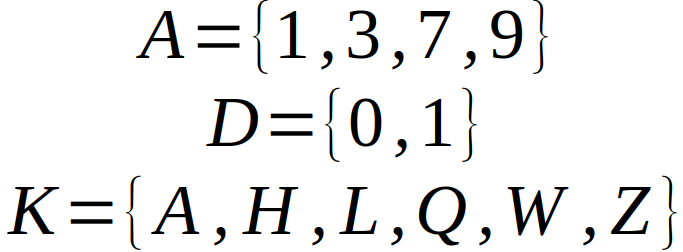
\includegraphics[width=40mm]{figures/sd_sets/enumeration_of_set.png}
	\end{center}}
\vspace{-4em}
\end{frame}

\begin{frame}%

	\begin{textitemize}
	\item by a defining expression describing the common characteristic property possessed by all and only the objects that are elements of (belong to) the set being specified
    \end{textitemize}

\vspace{2em}

	\scnrelfrom{illustration}{

		\begin{center}
			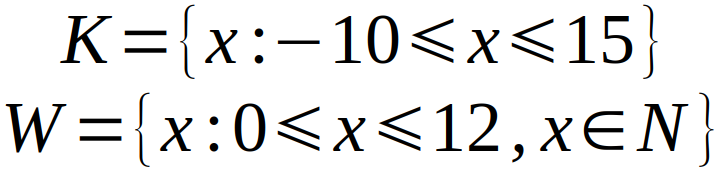
\includegraphics[width=45mm]{figures/sd_sets/descriptionProperties_set.png}
		\end{center}
	}
\vspace{-6em}
\end{frame}

\begin{frame}%

	\begin{textitemize}
	\item by set-theoretic operations that uniquely define new sets from existing ones, such as union, intersection and set difference
	\end{textitemize}

\vspace{2em}

    \scnrelfrom{illustration}{

	\begin{center}
		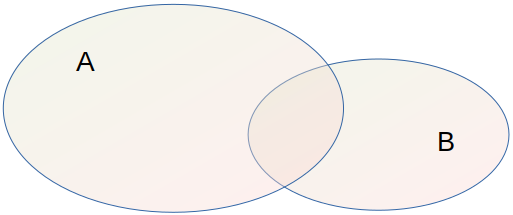
\includegraphics[width=40mm]{figures/sd_sets/unitiSets.png}
	\end{center}
     }

\vspace{0.2em}

    \scnrelfrom{illustration}{

	\begin{center}
		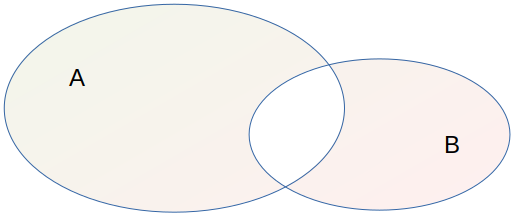
\includegraphics[width=40mm]{figures/sd_sets/intersectionSets.png}
	\end{center}
    }



	\vspace{-4em}
\end{frame}

\begin{frame}{\\Membership}
	\topline
	\justifying
	\begin{SCn}
		\scnheader{membership*}
		\scnidtf{membership of an element in a set*}
		\scniselement{binary relation}
		\scniselement{directed relation}
	\end{SCn}

	\textbf{\textit{membership*}} is a binary directed relation whose tuples connect a set to one of its elements.\\
	\bigskip
	The elements of the relation \textbf{\textit{membership*}} in \textit{SC-code} are, by default, \textbf{\textit{basic sc-arcs}} (positive permanent constant membership sc-arcs).
\end{frame}

\begin{frame}{\\Classification of sets}
	\topline
	\justifying
	\begin{SCn}
	\scnheader{set}
	\begin{scnrelfromset}{partition}
		\scnitem{finite set}
		\scnitem{infinite set}
	\end{scnrelfromset}
	\begin{scnrelfromset}{partition}
		\scnitem{set without repeated elements}
		\scnitem{multiset}
	\end{scnrelfromset}
	\begin{scnrelfromset}{partition}
		\scnitem{tuple}
		\scnitem{undirected set}
	\end{scnrelfromset}
	\end{SCn}
\end{frame}

\begin{frame}{\\Finiteness of sets}
	\topline
	\justifying
	\begin{SCn}
	\scnheader{finite set}
	\scnidtf{set with a finite number of elements}
	\end{SCn}

	\textbf{\textit{finite set}} is a \textit{set} whose number of elements is finite, i.e., there is a nonnegative integer \textit{k} equal to the number of elements in the set.
	\vspace{-\baselineskip}
	\begin{SCn}
	\scnheader{infinite set}
	\scnidtf{set with an infinite number of elements}
	\begin{scnrelfromset}{partition}
		\scnitem{countable set}
		\scnitem{uncountable set}
	\end{scnrelfromset}
	\end{SCn}
	\textbf{\textit{infinite set}} is a \textit{set} in which, for every natural number \textit{n} there is a finite subset with \textit{n} elements.

\end{frame}

\begin{frame}{\\Countability of sets}
	\topline
	\justifying
	\textbf{\textit{countable set}} is an \textit{infinite set} for which there is a \textit{one-to-one correspondence} with the natural numbers.

	\begin{SCn}
	\scnheader{uncountable set}
	\scnidtf{set of continuum cardinality}
	\end{SCn}

	\textbf{\textit{uncountable set}} is an \textit{infinite set} whose elements cannot be enumerated by natural numbers.
\end{frame}

\begin{frame}{\\Multiplicity of sets}%
	\topline
	\justifying
\begin{SCn}
	\scnheader{set without repeated elements}
	\scnidtf{classical set}
	\scnidtf{set consisting of distinct elements}
	\scntext{explanation}{\textbf{\textit{set without repeated elements}} is a \textit{set} for each element of which there is exactly one membership pair from the sign of the set to that element.}
\end{SCn}
\vspace{5.5em}
\end{frame}

\begin{frame}%
	\topline
	\justifying

	\begin{SCn}
		\scnheader{multiset}
		\scnidtf{set with multiple occurrences of at least one element}
		\scnidtf{set in which at least one element occurs more than once}
		\scntext{explanation}{\textbf{\textit{multiset}} is a \textit{set} for which there is at least one repeated membership pair originating from the sign of the set.}
	\end{SCn}

\end{frame}

\begin{frame}%
	\topline
	\justifying
	\vspace{10mm}
	\footnotesize
	\begin{SCn}
		\scnheader{membership multiplicity}
		\scnidtf{membership multiplicity of an element}
		\scnidtf{multiplicity of an element's occurrence in a set}
		\scniselement{parameter}
		\scntext{explanation}{\textbf{\textit{membership multiplicity}} -- \textit{parameter} whose values are numerical quantities indicating how many times an element occurs in the set. The elements of this parameter are classes of \textit{positive membership sc-arcs} connecting the set to the element whose multiplicity we wish to specify.

Repeated occurrence of an element in a multiset can therefore be represented either by explicitly specifying the \textit{positive membership sc-arcs} of this element in the \textit{set} or by ``merging''{} these arcs into one and including it in a class of \textbf{\textit{membership multiplicity}}.}
	\end{SCn}


\end{frame}

\begin{frame}%
\scnrelfrom{example description}{
	\begin{center}
	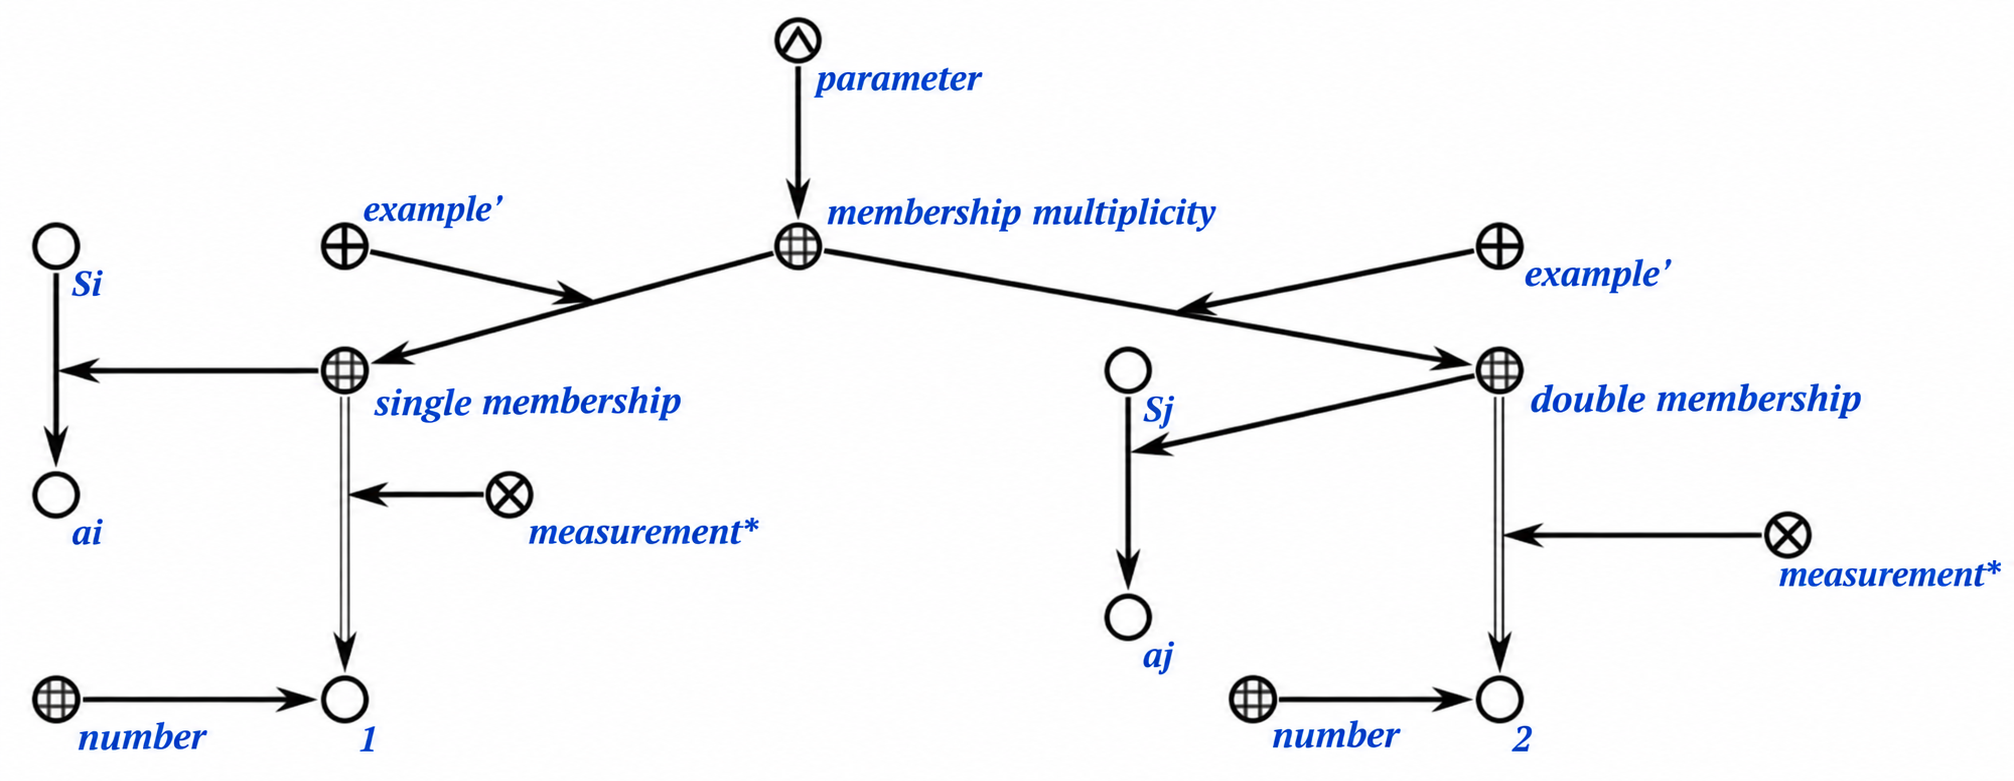
\includegraphics[width=120mm]{figures/sd_sets/multiplicityOfMembership_en.png}
	\end{center}
}
\vspace{-1em}
\end{frame}

\begin{frame}{\\Fuzzy and crisp sets }%
\topline
\justifying
\vspace{10mm}
	\begin{SCn}
\scnheader{fuzzy set}
\scntext{explanation}{\textbf{\textit{fuzzy set}} is a \textit{set} that is a collection of elements of arbitrary nature for which it cannot be stated with certainty whether they possess the characteristic property used to define this fuzzy set. Membership in such a set is specified using \textit{fuzzy positive membership sc-arcs}.}

\scnheader{crisp set}
\scntext{explanation}{\textbf{\textit{crisp set}} is a \textit{set} whose element membership is certain and is specified using \textit{crisp positive membership sc-arcs}.}
\end{SCn}

\end{frame}

\begin{frame}{\\Family of sets}%
	\topline
	\justifying
	\begin{SCn}
		\scnheader{family of sets}
		\scnidtf{set of sets}
		\scnsuperset{class of classes}

	\scntext{explanation}{\textbf{\textit{family of sets}} is a \textit{set} whose elements are signs of sets.}
		\end{SCn}

\end{frame}

\begin{frame}{\\Properties of relations on a set}%
	\topline
	\justifying

\begin{SCn}
\scnheader{non-reflexive set}
\scntext{explanation}{\textbf{\textit{non-reflexive set}} is a \textit{set} whose sign is not an element of the set}

\scnheader{reflexive set}
\scntext{explanation}{\textbf{\textit{reflexive set}} is a \textit{set} whose sign is an element of the set}
\end{SCn}

\vspace{-1em}
\end{frame}

\begin{frame}{\\Cardinality}%
	\topline
	\justifying

	\begin{SCn}
		\scnheader{cardinality of a set}
		\scnidtf{cardinal number}
		\scnidtf{total number of element occurrences in a given set}
		\scnidtf{equivalence class whose elements are the signs of all and only the sets with the same cardinality}
		\scnidtf{equivalence class corresponding to the relation of being a pair of sets of equal cardinality (equicardinality of sets)}
		\scnidtf{set cardinality quantity}
		\scnidtf{transfinite number}
		\scnidtf{Cantorian cardinality}
		\scniselement{parameter}
	\end{SCn}
\end{frame}

\begin{frame}{\\Cardinality}%
	\topline
	\justifying
	\begin{SCn}
	\scnheader{cardinality of a set}
	\scntext{explanation}{\textbf{\textit{cardinality of a set}} is a \textit{parameter} whose elements are \textit{sets} with the same number of elements. The value of this parameter is a numerical quantity specifying the number of elements in the given class of sets, i.e., essentially, the number of \textit{positive membership sc-arcs} originating from the given \textit{set}.}

	\scnheader{set}
	\scnsuperset{empty set}
	\scnsuperset{singleton}
	\scnsuperset{pair}
	\scnsuperset{triple}
	\end{SCn}
	\vspace{-2em}
\end{frame}

\begin{frame}{\\Empty set} %
  \topline
  \justifying

   \begin{SCn}
	\scnheader{empty set}
	\scniselement{cardinality of a set}
    \scntext{explanation}{\textbf{\textit{empty set}} is a \textit{set} to which no element belongs.}
    \end{SCn}

\vspace{8.5em}
\end{frame}

\begin{frame}{\\Singleton}%
	\topline
	\justifying

	\begin{SCn}
	\scnheader{singleton}
	\scniselement{cardinality of a set}
	\scnidtf{set of cardinality 1}
	\scnidtf{one-element set}
	\scnidtf{set of cardinality one}
    \scnidtf{set whose cardinality equals 1}
    \scnidtf{set with cardinality equal to one}
    \scnidtf{singleton of an sc-element}
    \scnidtf{sc-singleton}
    \scnsubset{finite set}
	\scntext{explanation}{\textbf{\textit{singleton}} is a \textit{set} consisting of one element.}
	\end{SCn}

\end{frame}

\begin{frame}{\\Pair}%
	\topline
\justifying
    \begin{SCn}
	\scnheader{pair}
	\scniselement{cardinality of a set}
	\scnidtf{set of cardinality two}
	\scnidtf{two-element set}
	\scnidtf{set of cardinality 2}
	\scnsubset{finite set}
    \scntext{explanation}{\textbf{\textit{pair}} is a \textit{set} consisting of two elements.}
    \end{SCn}
\vspace{4.5em}

\end{frame}

\begin{frame}{\\Triple} %
	\topline
\justifying

	\begin{SCn}
	\scnheader{triple}
	\scniselement{cardinality of a set}
	\scnidtf{triple}
	\scnidtf{set of cardinality three}
	\scnsubset{finite set}
	\scntext{explanation}{\textbf{\textit{triple}} is a \textit{set} consisting of three elements.}
	\end{SCn}


\end{frame}



\begin{frame}{\\Tuple}%
	\topline
\justifying

	\begin{SCn}
    \scnheader{tuple}
    \scnidtf{vector}
    \scntext{explanation}{\textbf{\textit{tuple}} is a set representing an ordered collection of elements, i.e., a set in which the order of the elements matters. The membership pairs of elements of a \textbf{\textit{tuple}} may additionally belong to \textit{role relations}; within each \textbf{\textit{tuple}} there must be at least one element whose role is further specified by a \textit{role relation}.}
	\end{SCn}

\vspace{2em}
\end{frame}

\begin{frame}
	\centering
	\Huge
	\textbf{Relations on sets}
\end{frame}

%
\begin{frame}{\\Relations on sets}%
\topline
\justifying
	\begin{SCn}
    \scnheader{inclusion*}
    \scnidtf{be a subset*}
    \scniselement{binary relation}
    \scniselement{directed relation}
    \scniselement{transitive relation}
    \scnrelfrom{domain of definition}{set}
    \scnsuperset{strict inclusion*}
    \scntext{definition}{\textbf{\textit{inclusion*}} is a binary directed relation whose tuples connect two sets. We say that \textit{Set Si} \textbf{\textit{includes*}} \textit{Set Sj} as a subset if and only if every element of \textit{Set Sj} is also an element of \textit{Set Si}.}
	\end{SCn}
    \vspace{-3em}
\end{frame}

\begin{frame}%
    \scnrelfrom{example description}{
    \begin{center}
	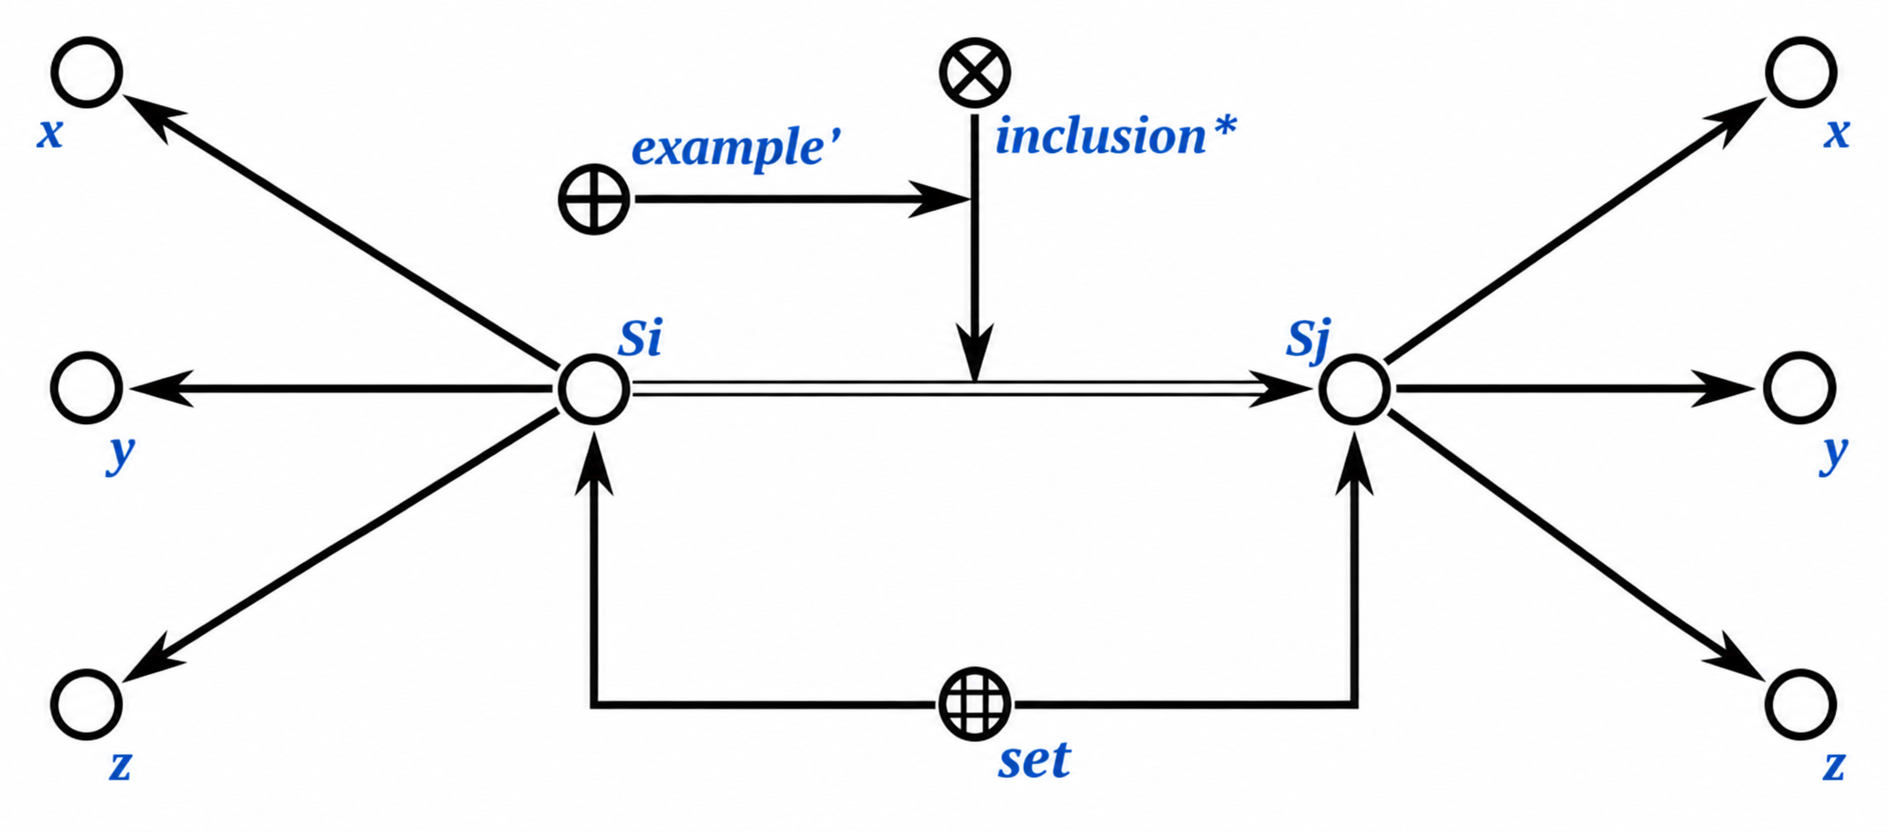
\includegraphics[width=100mm]{figures/sd_sets/inclusion_en.png}
    \end{center}}


    \begin{scnindent}
    \scntext{explanation}{Set \textbf{\textit{Sj}} is included in set \textbf{\textit{Si}}.}
    \end{scnindent}
\vspace{-1em}
\end{frame}

\begin{frame}%
	\topline
	\justifying
	\vspace{10mm}
	\footnotesize
	\begin{SCn}
	\scnheader{strict inclusion*}
	\scnidtf{strict inclusion of sets*}
	\scnsubset{inclusion*}
	\scniselement{binary relation}
	\scniselement{directed relation}
	\scnrelfrom{domain of definition}{set}
    \scntext{definition}{\textbf{\textit{strict inclusion*}} is a \textit{binary directed relation} whose domain of definition is the family of all sets. We say that \textit{Set Si} \textbf{\textit{strictly includes*}} \textit{Set Sj} as a subset if and only if every element of \textit{Set Sj} is also an element of \textit{Set Si} and there is at least one element of \textit{Set Si} that is not an element of \textit{Set Sj}.}
	\end{SCn}
    \vspace{3em}
\end{frame}

\begin{frame}%

    \scnrelfrom{example description}{
	\begin{center}
	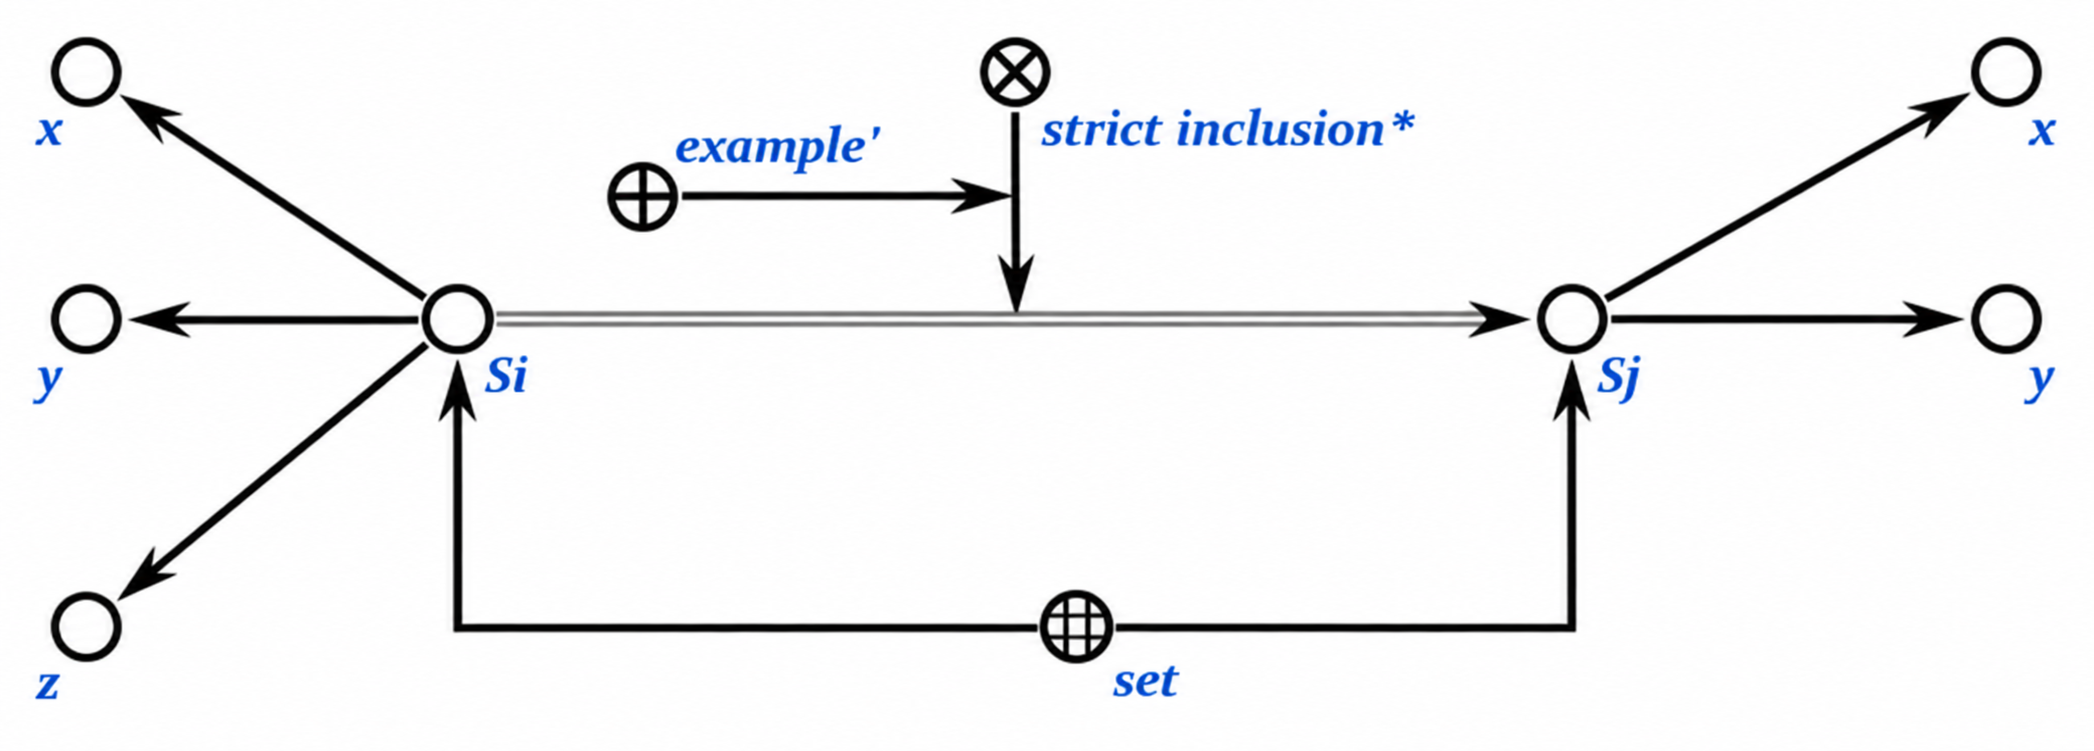
\includegraphics[width=22em]{figures/sd_sets/strictInclusion_en.png}
    \end{center}}

    \begin{scnindent}
    \scntext{explanation}{Set \textit{Sj} is strictly included in set \textit{Si}.}
    \end{scnindent}

\scnrelfrom{illustration}{
	\begin{center}
		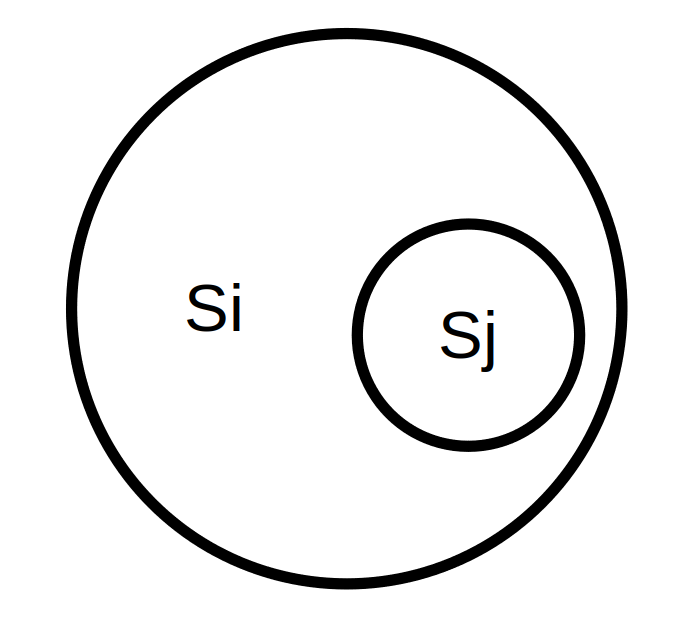
\includegraphics[width=7em]{figures/sd_sets/inclusion2.png}
\end{center}}

\vspace{-1.5em}
\end{frame}

\begin{frame}%
	\topline
	\justifying
	\vspace{10mm}

	\begin{SCn}
		\scnheader{equality of sets*}
		\scniselement{binary relation}
		\scniselement{undirected relation}
		\scnidtf{be equal sets*}

	    \scntext{definition}{\textbf{\textit{equality of sets}}* is a binary undirected relation expressing equality of sets.
Two sets are equal if and only if the first includes the second and the second includes the first.}
	\end{SCn}

\end{frame}

\begin{frame}%
    \scnrelfrom{example description}{
    \begin{center}
%
	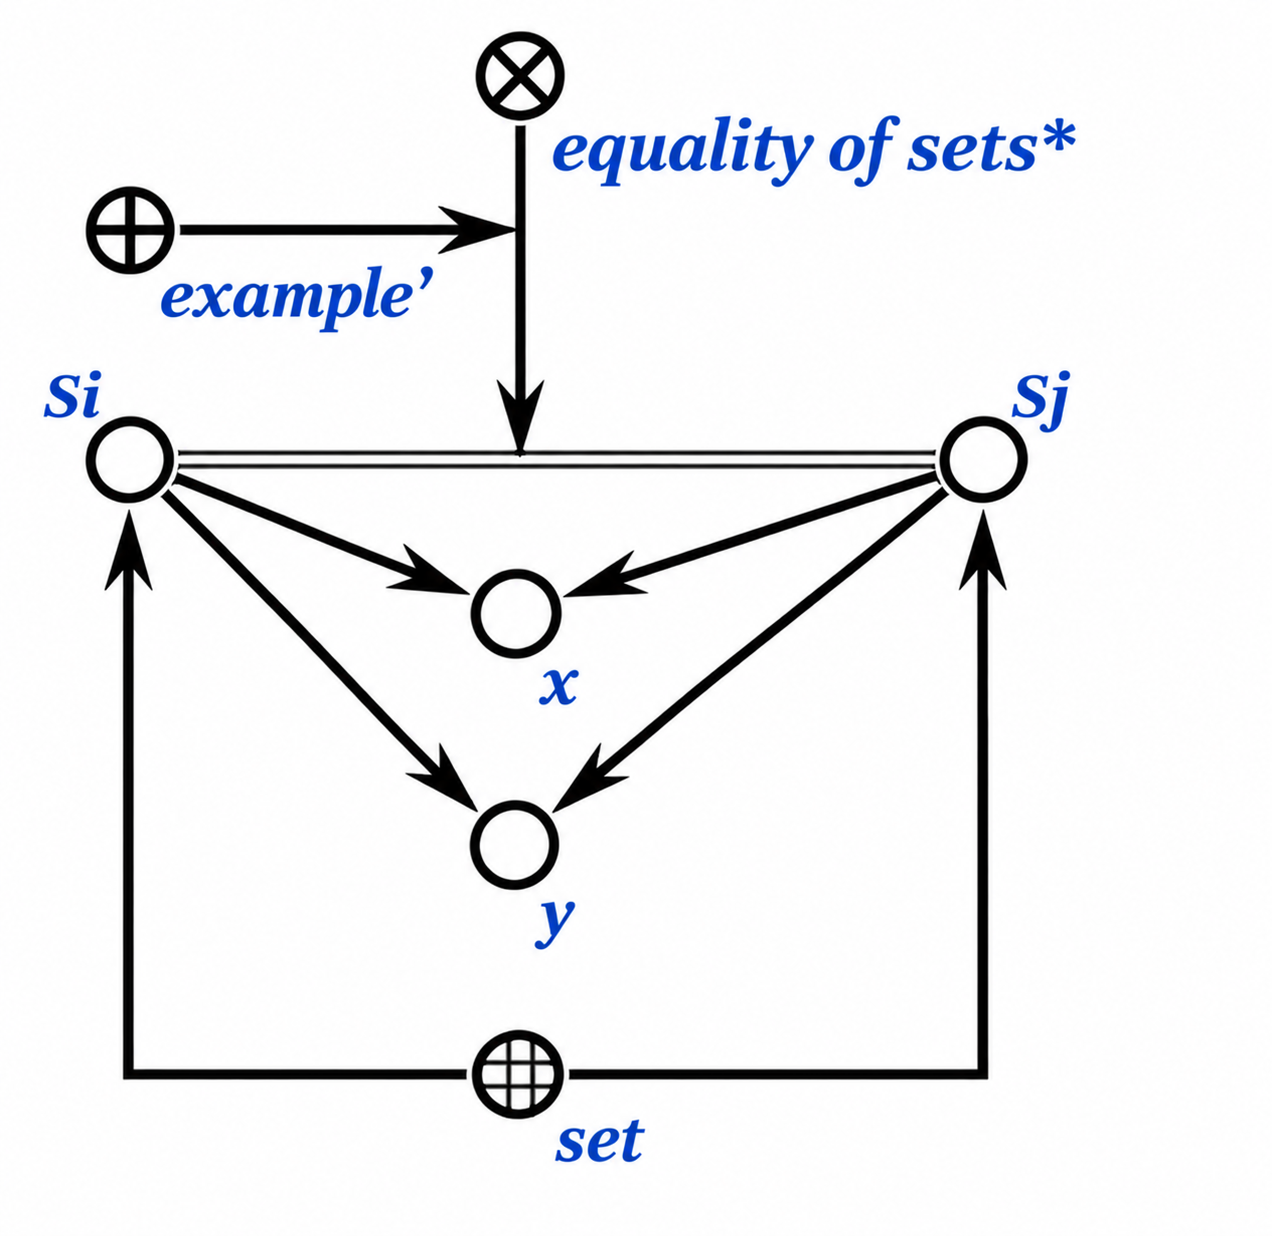
\includegraphics[width=50mm]{figures/sd_sets/equalityOfSets_en.png}
    \end{center}}

    \begin{scnindent}
    \scntext{explanation}{Set \textit{Si} is equal to set \textit{Sj}.}
    \end{scnindent}

\end{frame}

\begin{frame}%
	\topline
	\justifying
	\vspace{5mm}
	\footnotesize

	\begin{SCn}
		\scnheader{power set*}
		\scnidtf{power set of a set*}
		\scnidtf{family of all subsets of a given set*}
		\scniselement{binary relation}
		\scniselement{directed relation}

    \scntext{definition}{\textbf{\textit{power set*}} is a \textit{binary directed relation} between a set and a family of sets each of which is a subset of the first set.}

    \scnrelfrom{example description}{
    \begin{center}
    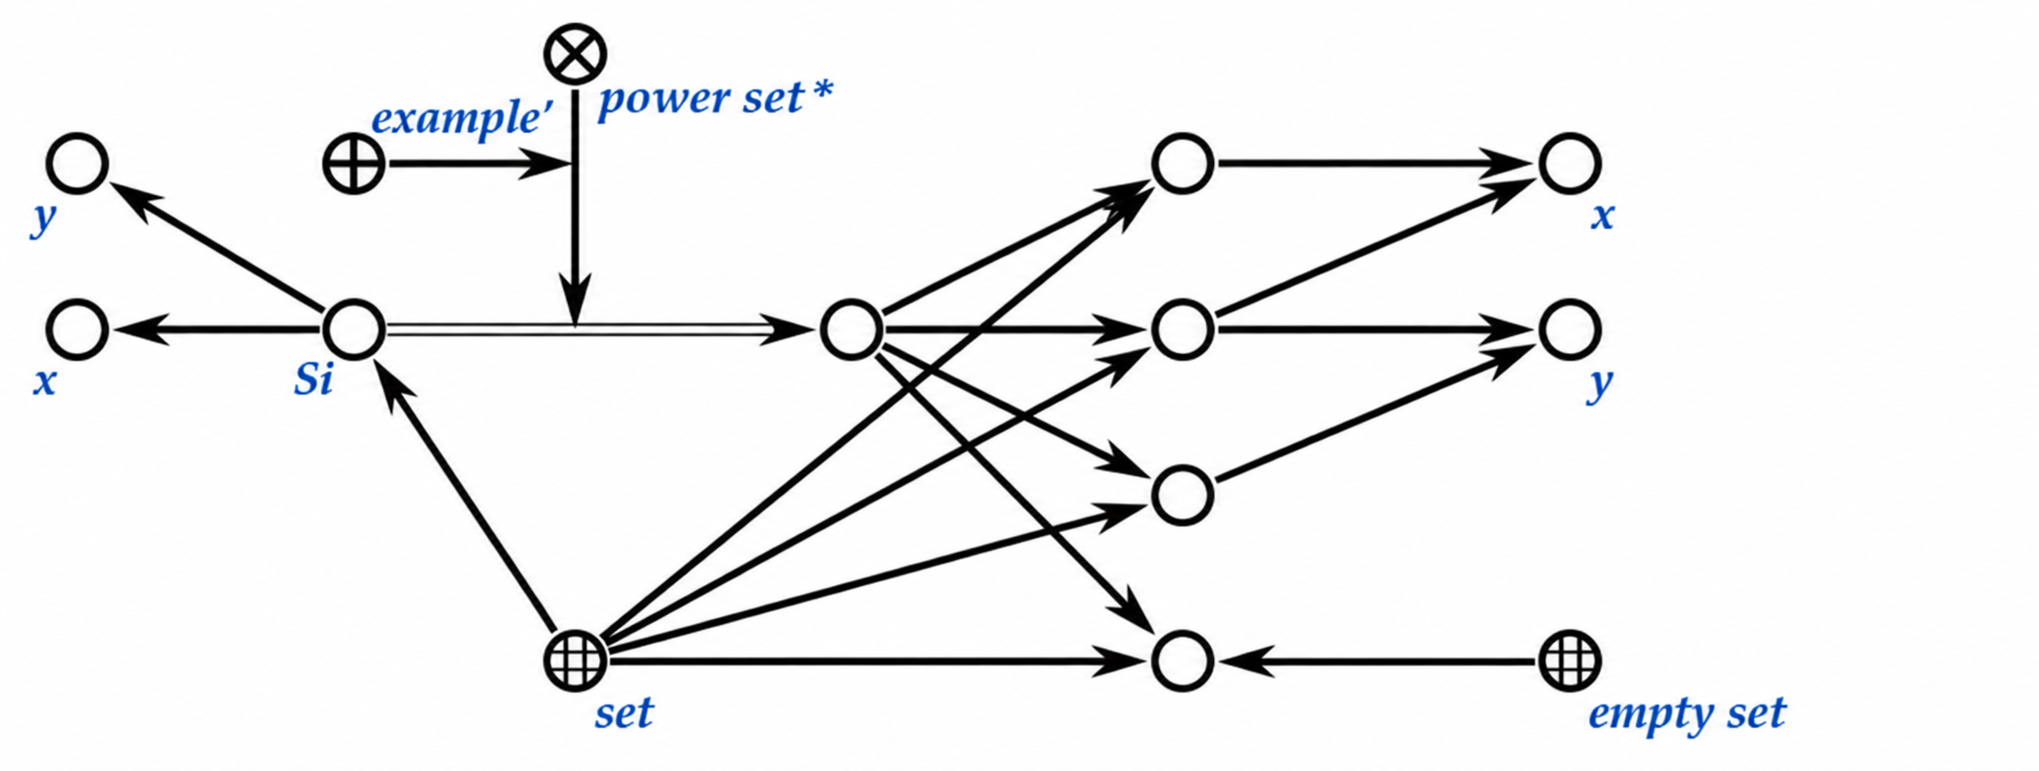
\includegraphics[width=100mm]{figures/sd_sets/boulean_en.png}
    \end{center}}
	\end{SCn}

\end{frame}

\begin{frame}%
\topline
\justifying
\vspace{5mm}
   \footnotesize
   \begin{SCn}
	\scnheader{family of subsets*}
	\scnidtf{family of subsets of a given set*}
	\scniselement{binary relation}
	\scniselement{directed relation}
	\scnsuperset{power set*}

    \scntext{definition}{\textbf{\textit{family of subsets*}} is a \textit{binary directed relation} between a set and a family of sets each of which is a subset of the first set.}

    \scnrelfrom{example description}{
    \begin{center}
    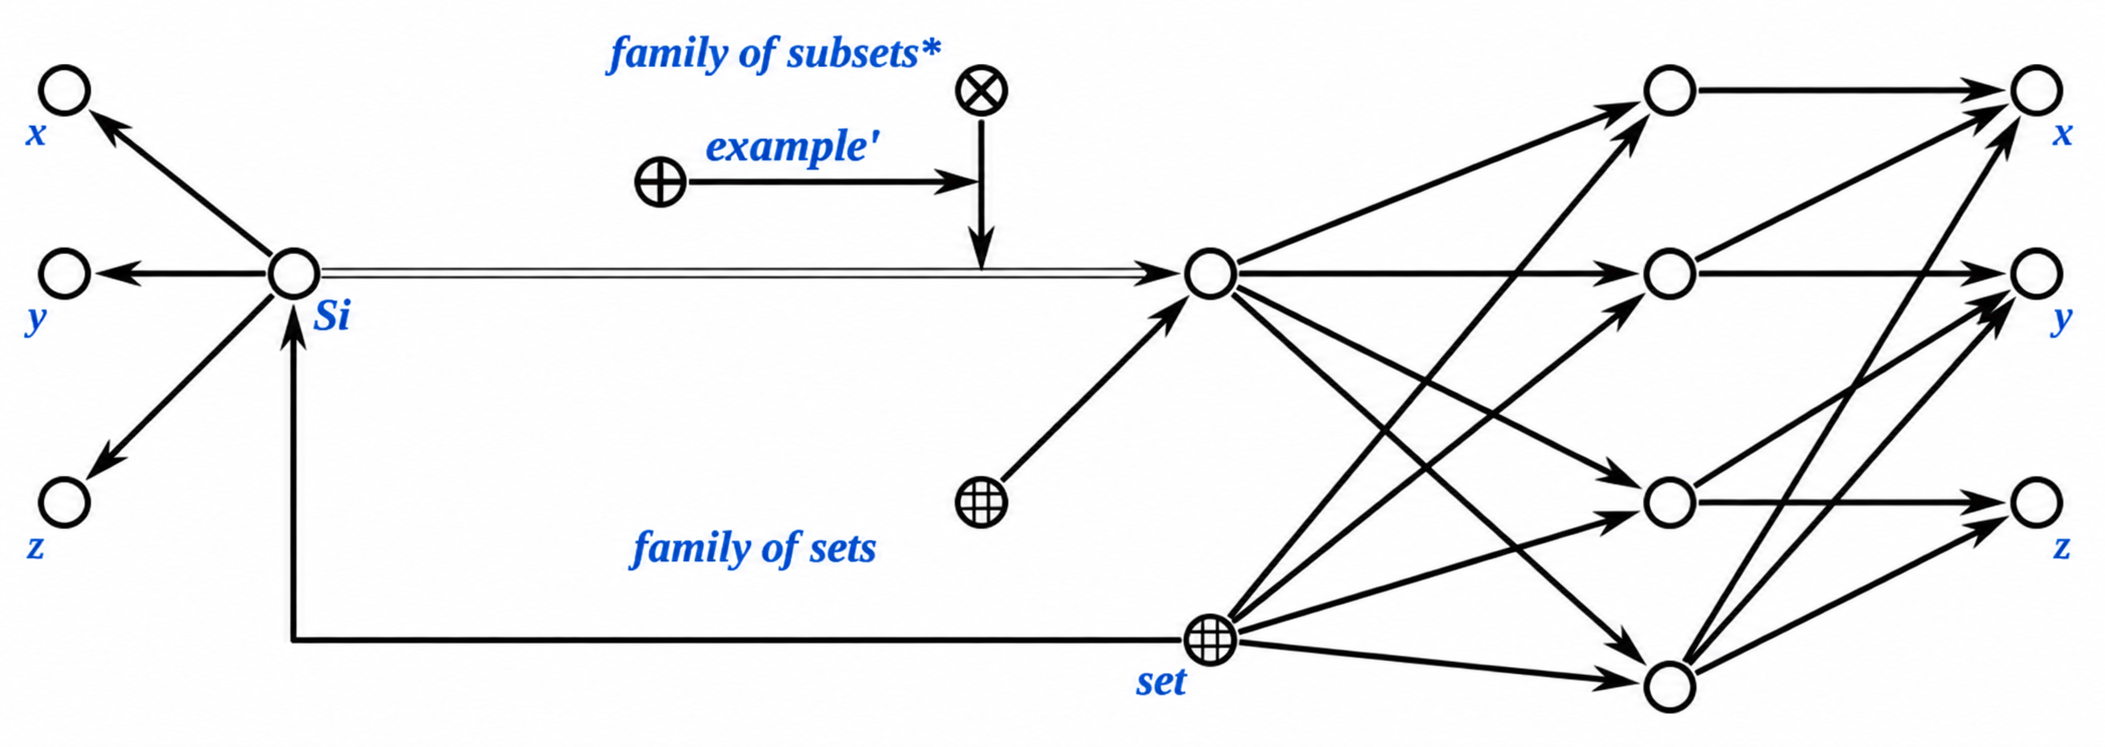
\includegraphics[width=100mm]{figures/sd_sets/familyOfSubsets_en.png}
    \end{center}}
	\end{SCn}

\end{frame}

%
\begin{frame}{\\Operations on sets}%
\topline
\justifying
	\begin{SCn}
		\scnheader{union*}
		\scnidtf{union of sets*}
		\scniselement{quasi-binary relation}
		\scniselement{directed relation}

    \scntext{definition}{\textbf{\textit{union*}} is a \textit{quasi-binary directed relation} whose domain of definition is the family of all sets. We say that \textit{Set Si} is the union of \textit{Set Sj} and \textit{Set Sk} if and only if every element of \textit{Set Si} is an element of either \textit{Set Sj} or \textit{Set Sk}.}
    \end{SCn}

    \vspace{1em}

\end{frame}

\begin{frame}%

  \scnrelfrom{example description}{
	\begin{center}
		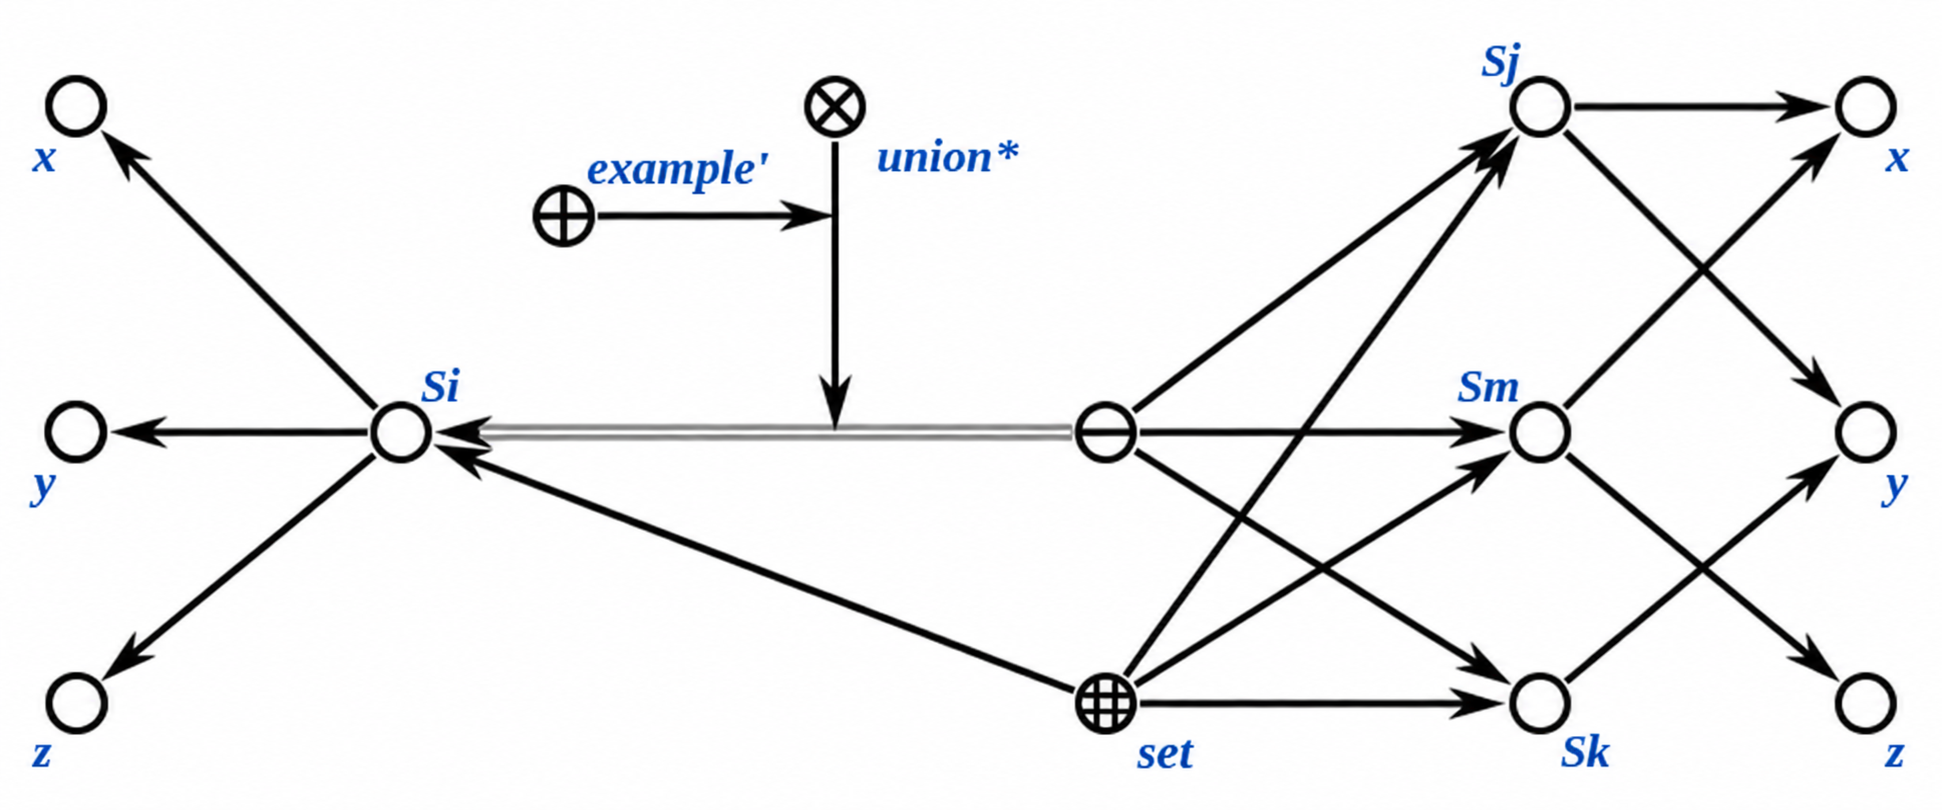
\includegraphics[width=75mm]{figures/sd_sets/union_en.png}
 \end{center}}
    \begin{scnindent}
	\scntext{explanation}{Set \textit{Si} is the union of sets \textit{Sj}, \textit{Sk} and \textit{Sm}.}
    \end{scnindent}

    \scnrelfrom{illustration}{
    \begin{center}
    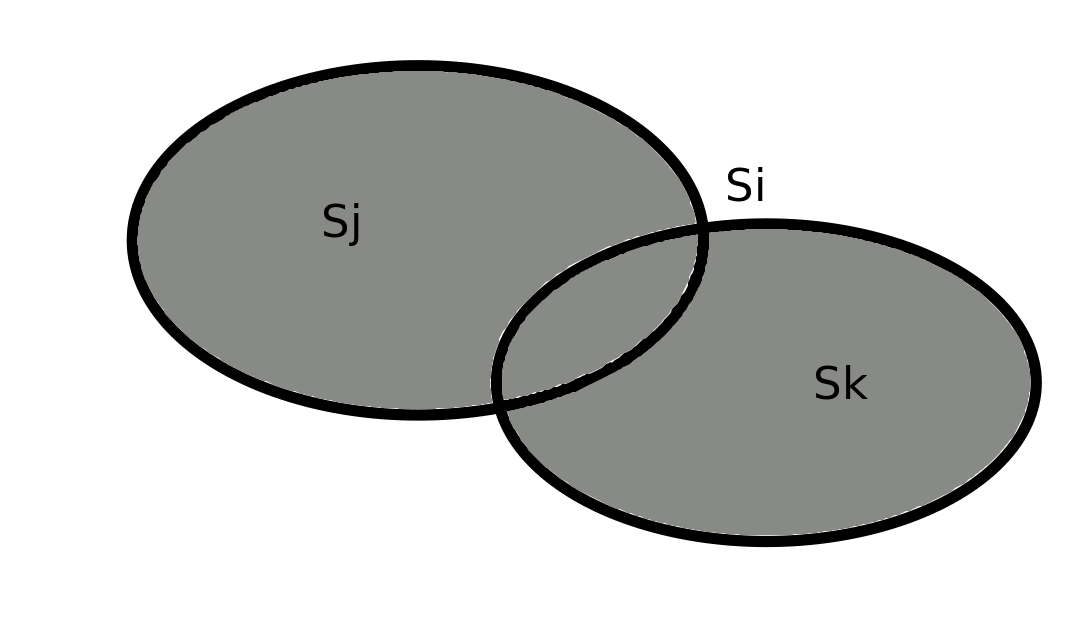
\includegraphics[width=45mm]{figures/sd_sets/union2.png}
    \end{center}}
\vspace{-3em}
\end{frame}

%
\begin{frame}%
\topline
\justifying

	\begin{SCn}
	\scnheader{partition*}
	\scnidtf{partition of a set*}
	\scnidtf{union of pairwise disjoint sets*}
	\scnidtf{decomposition of a set*}
	\scniselement{quasi-binary relation}
	\scniselement{directed relation}
	\scniselement{decomposition relation}
	\end{SCn}
\end{frame}

\begin{frame}
\topline
\justifying
\vspace{10mm}
\footnotesize
	\begin{SCn}
	\scnheader{partition*}
\scntext{definition}{\textbf{\textit{partition*}} is a \textit{quasi-binary directed relation} whose domain of definition is the family of all sets. Partitioning a set produces a family of pairwise disjoint sets whose union is the original set.

The family of sets \{\textit{S1, \ldots, Sn}\} is a partition of set \textit{Si} if and only if:

	\begin{textitemize}
		\item the family \{\textit{S1, \ldots, Sn}\} is a family of \textit{pairwise disjoint sets};
		\item the family \{\textit{S1, \ldots, Sn}\} is a cover of set \textit{Si} (the set \textit{Si} is the \textit{union} of the sets in the above family)
	\end{textitemize}}
\end{SCn}
\end{frame}

\begin{frame}%

    \scnrelfrom{example description}{
    \begin{center}
    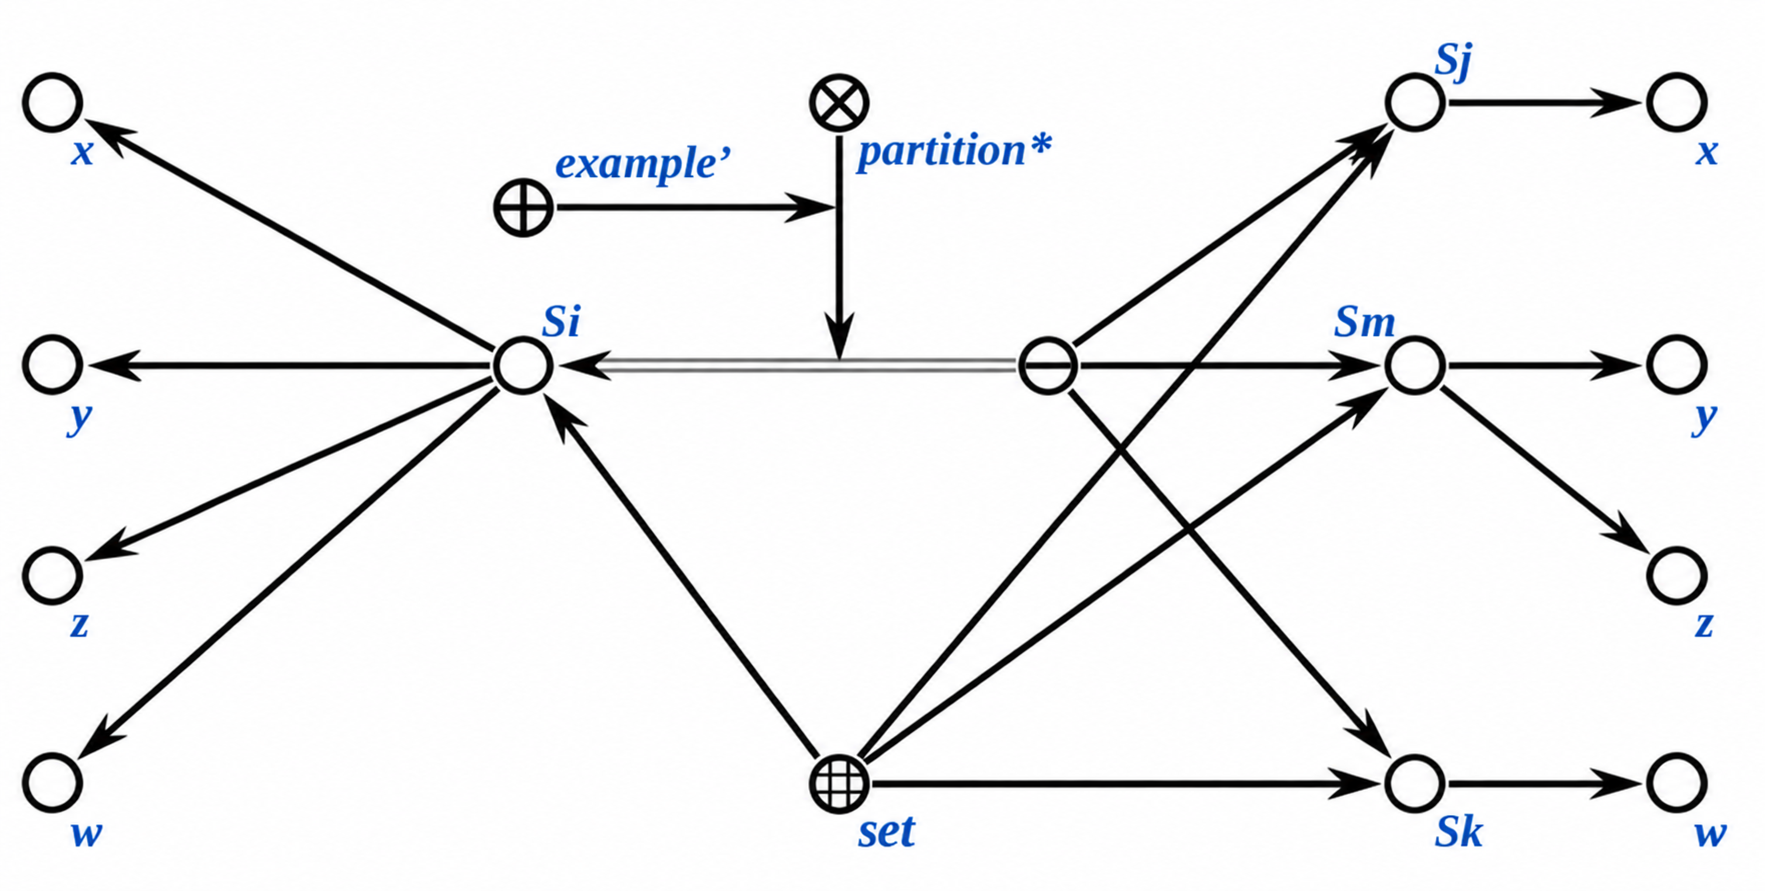
\includegraphics[width=60mm]{figures/sd_sets/split_en.png}
    \end{center}}

    \begin{scnindent}
    \scntext{explanation}{Set \textit{Si} is partitioned into sets \textit{Sj}, \textit{Sk} and \textit{Sm}.}
    \end{scnindent}

    \scnrelfrom{illustration}{
    \begin{center}
	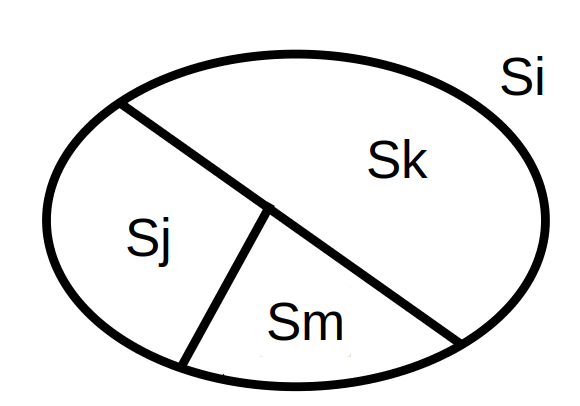
\includegraphics[width=40mm]{figures/sd_sets/split2.png}
    \end{center}}

\end{frame}

\begin{frame}%
\topline
\justifying
\vspace{10mm}

	\begin{SCn}
	\scnheader{intersection*}
	\scnidtf{intersection of sets*}
	\scniselement{quasi-binary relation}
	\scniselement{directed relation}
	\end{SCn}

    \scntext{definition}{\textbf{\textit{intersection*}} is an operation on two or more sets whose result contains exactly the entities that belong simultaneously to every set in the family of arguments.\\
We say that \textit{Set Si} is the intersection of \textit{Set Sj} and \textit{Set Sk} if and only if every element of \textit{Set Si} is an element of \textit{Set Sj} and an element of \textit{Set Sk}.}

\end{frame}

\begin{frame}%

    \scnrelfrom{example description}{
    \begin{center}
	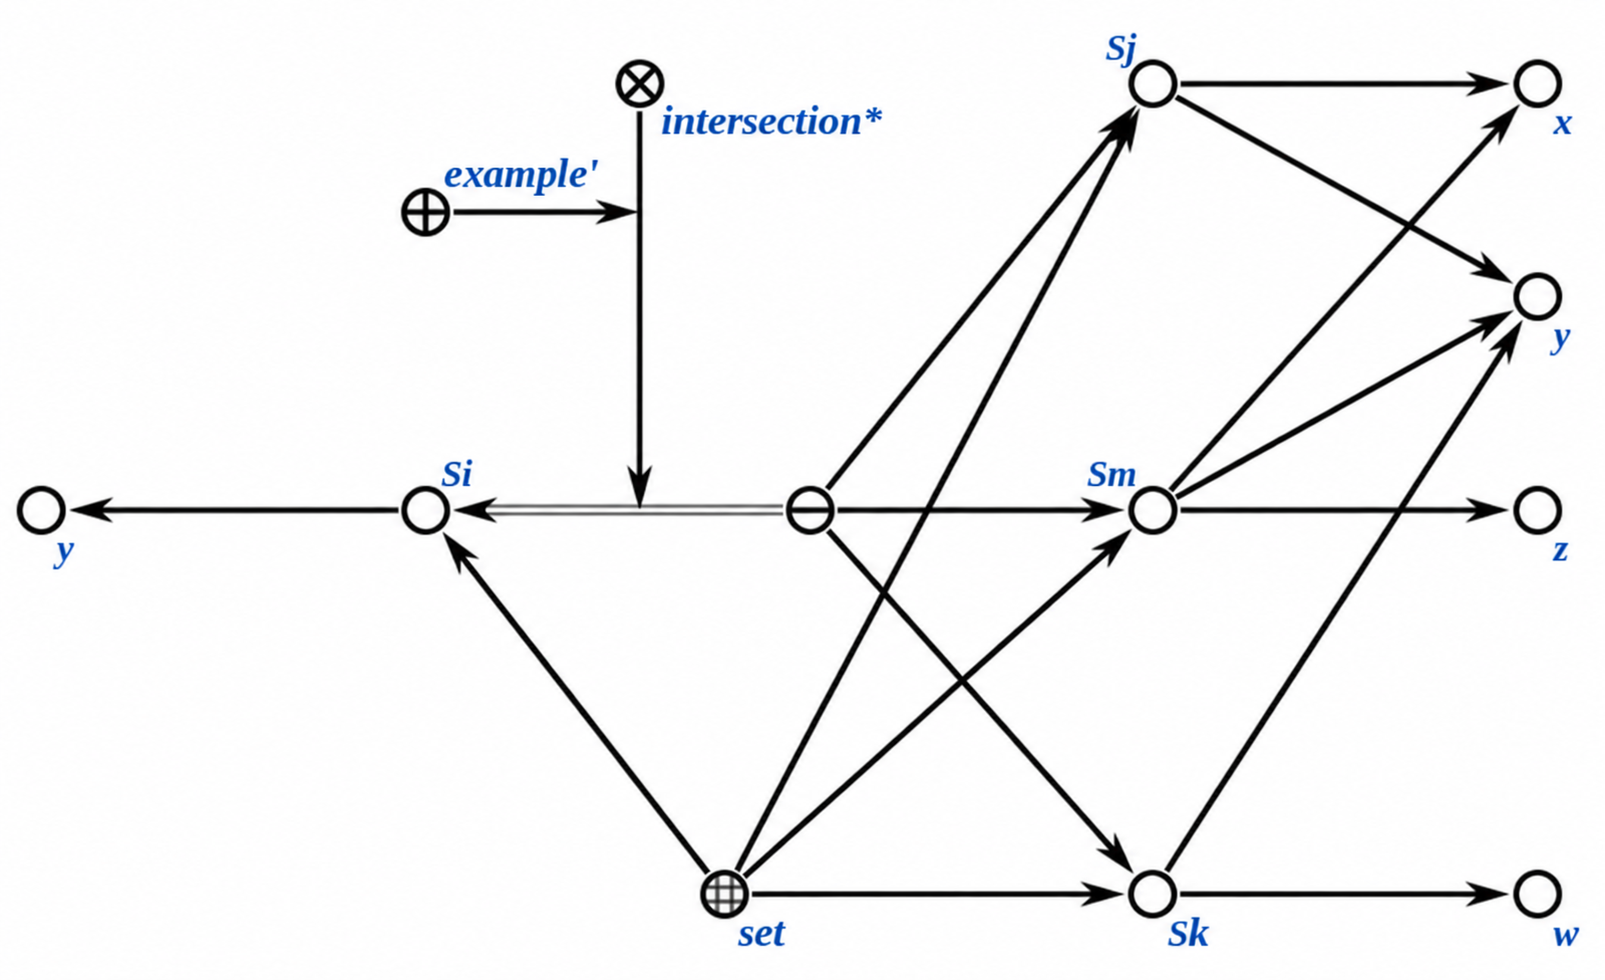
\includegraphics[width=70mm]{figures/sd_sets/intersection_en.png}
    \end{center}}

    \begin{scnindent}
    \scntext{explanation}{Set \textit{Si} is the intersection of sets \textit{Sj}, \textit{Sk} and \textit{Sm}.}
    \end{scnindent}

    \scnrelfrom{illustration}{
    \begin{center}
	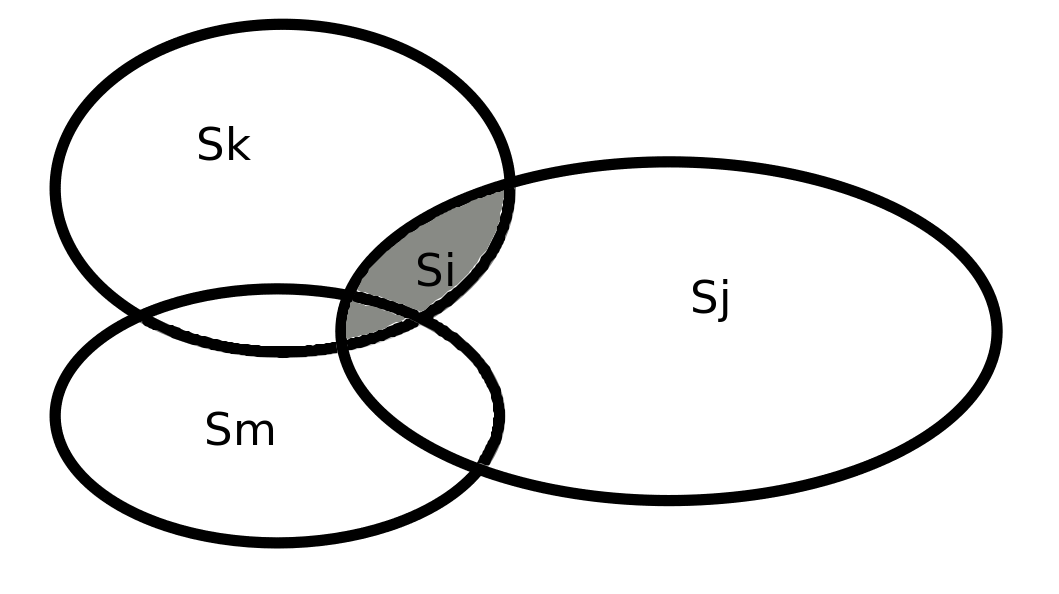
\includegraphics[width=40mm]{figures/sd_sets/intersection2.png}
    \end{center}}

\end{frame}

\begin{frame}%
\topline
\justifying
\vspace{10mm}

	\begin{SCn}
	\scnheader{set difference*}
	\scniselement{binary relation}
	\scniselement{directed relation}
	\scntext{definition}{\textbf{\textit{set difference*}} is a \textit{binary directed relation} that connects an \textit{ordered pair} whose first element is the minuend set and whose second element is the subtrahend set, to their difference: the set of all elements of the first set that do not belong to the second set.}
	\end{SCn}


\end{frame}

\begin{frame}%

   \scnrelfrom{example description}{
   \begin{center}
   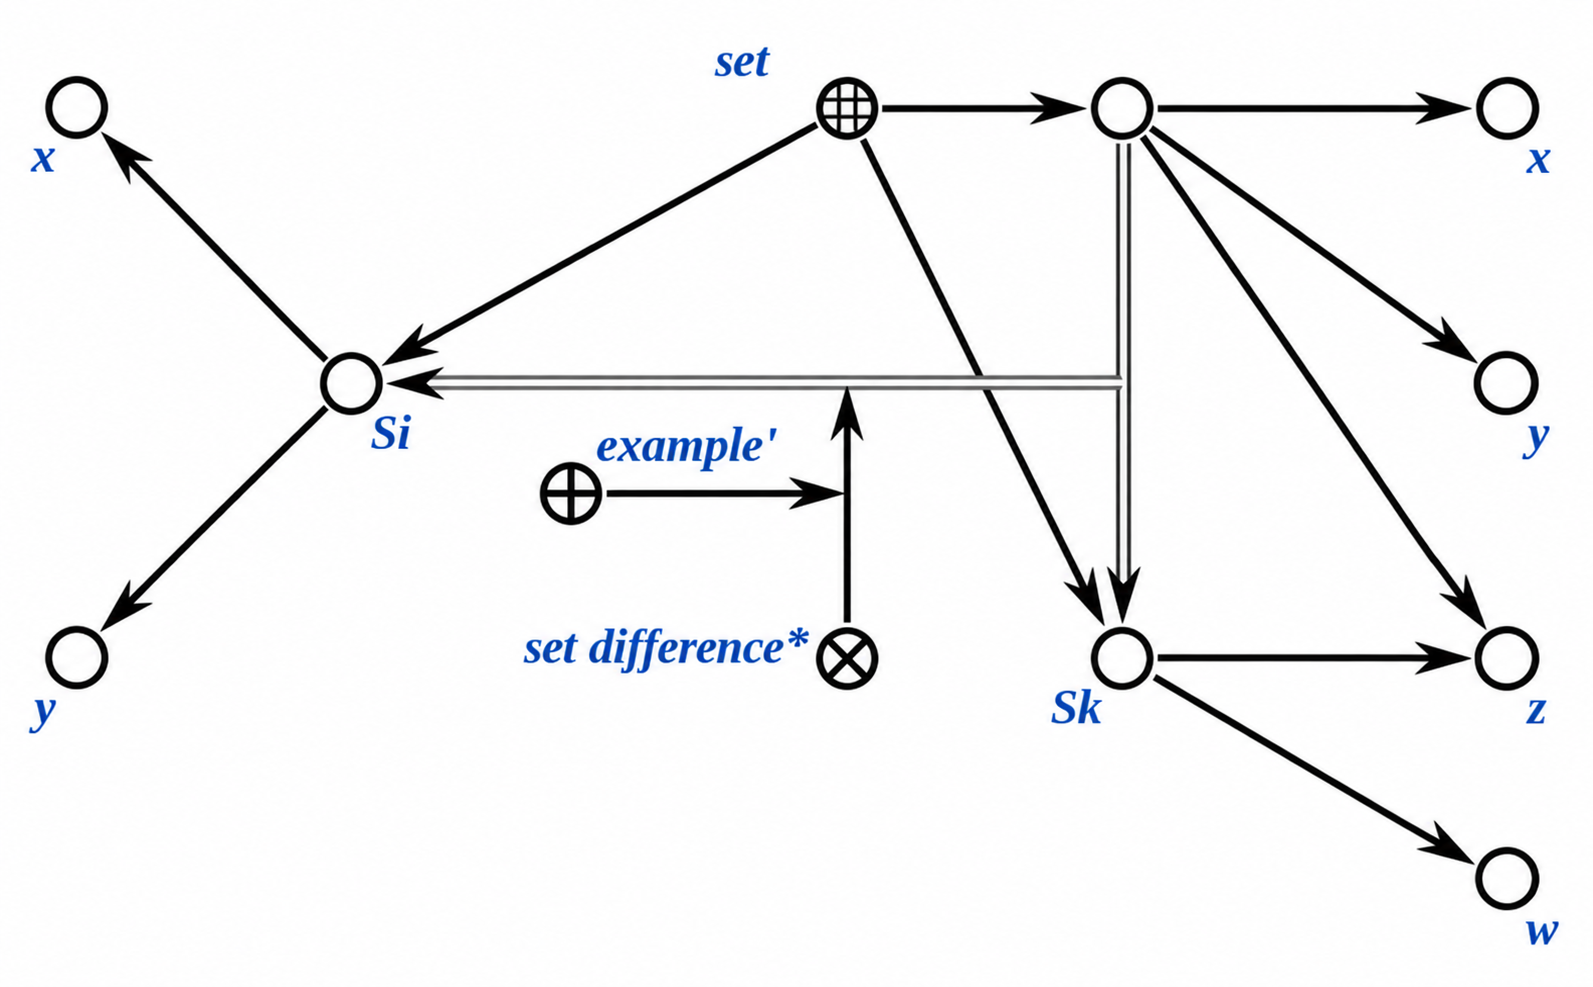
\includegraphics[width=75mm]{figures/sd_sets/setDifference_en.png}
   \end{center}}

   \begin{scnindent}
   \scntext{explanation}{Set \textit{Si} is the difference of sets \textit{Sj} and \textit{Sk}.}
   \end{scnindent}

   \scnrelfrom{illustration}{
   \begin{center}
   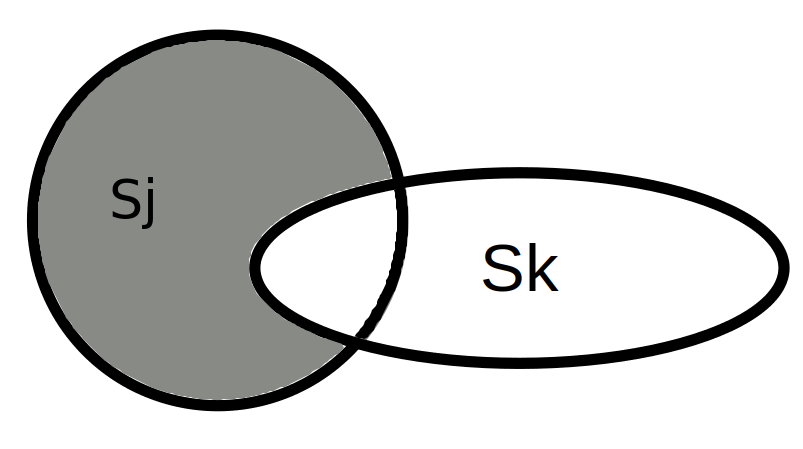
\includegraphics[width=37mm]{figures/sd_sets/setDifference2.png}
   \end{center}}

\end{frame}

\begin{frame}%
\topline
\justifying
\vspace{10mm}

	\begin{SCn}
	\scnheader{symmetric difference of sets*}
	\scniselement{binary relation}
	\scniselement{directed relation}

    \scntext{definition}{\textbf{\textit{symmetric difference of sets*}} is a \textit{binary directed relation} that connects a \textit{pair} of sets to the set that is their symmetric difference. We call \textit{Set Si} the symmetric difference of \textit{Set Sj} and \textit{Set Sk} if and only if every element of \textit{Set Si} is an element of either \textit{Set Sj} or \textit{Set Sk} but is not an element of both sets.}
	\end{SCn}

\end{frame}

\begin{frame}%

    \scnrelfrom{example description}{
    \begin{center}
	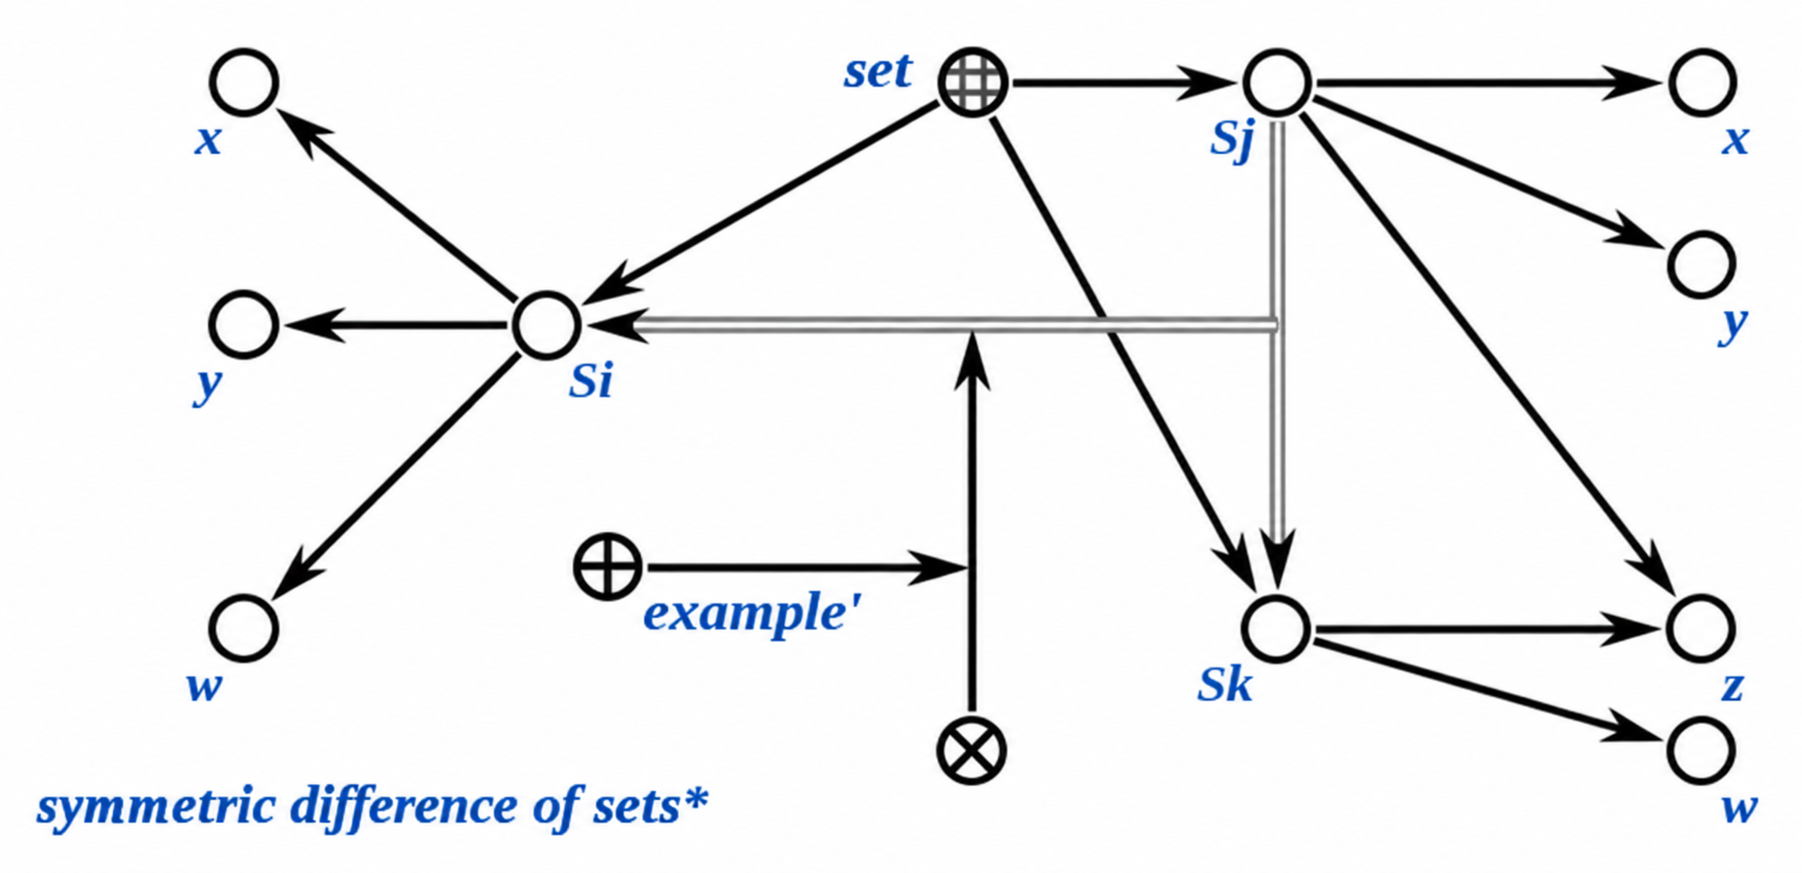
\includegraphics[width=75mm]{figures/sd_sets/symmetricDifferenceOfSets_en.png}
	\end{center}}

	\scntext{explanation}{Set \textit{Si} is the symmetric difference of sets \textit{Sj} and \textit{Sk}.}

    \scnrelfrom{illustration}{
    \begin{center}
	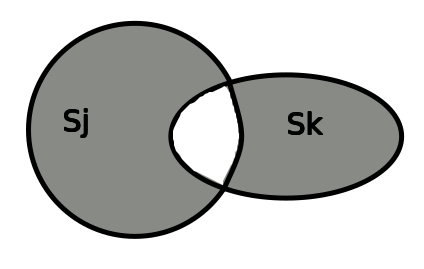
\includegraphics[width=35mm]{figures/sd_sets/symmetricDifferenceOfSets2.png}
    \end{center}}

\end{frame}

\begin{frame}%
\topline
\justifying
\vspace{10mm}

	\begin{SCn}
	\scnheader{Cartesian product*}
	\scnidtf{Cartesian product of sets*}
	\scnidtf{direct product of sets*}
	\scniselement{binary relation}
	\scniselement{directed relation}
    \scntext{definition}{\textbf{\textit{Cartesian product*}} is a \textit{binary directed relation} between an \textit{ordered pair} of sets and a \textit{set} whose elements are all ordered pairs with a first component from the first set and a second component from the second set.}
	\end{SCn}


\end{frame}

\begin{frame}%

    \scnrelfrom{example description}{
    \begin{center}
	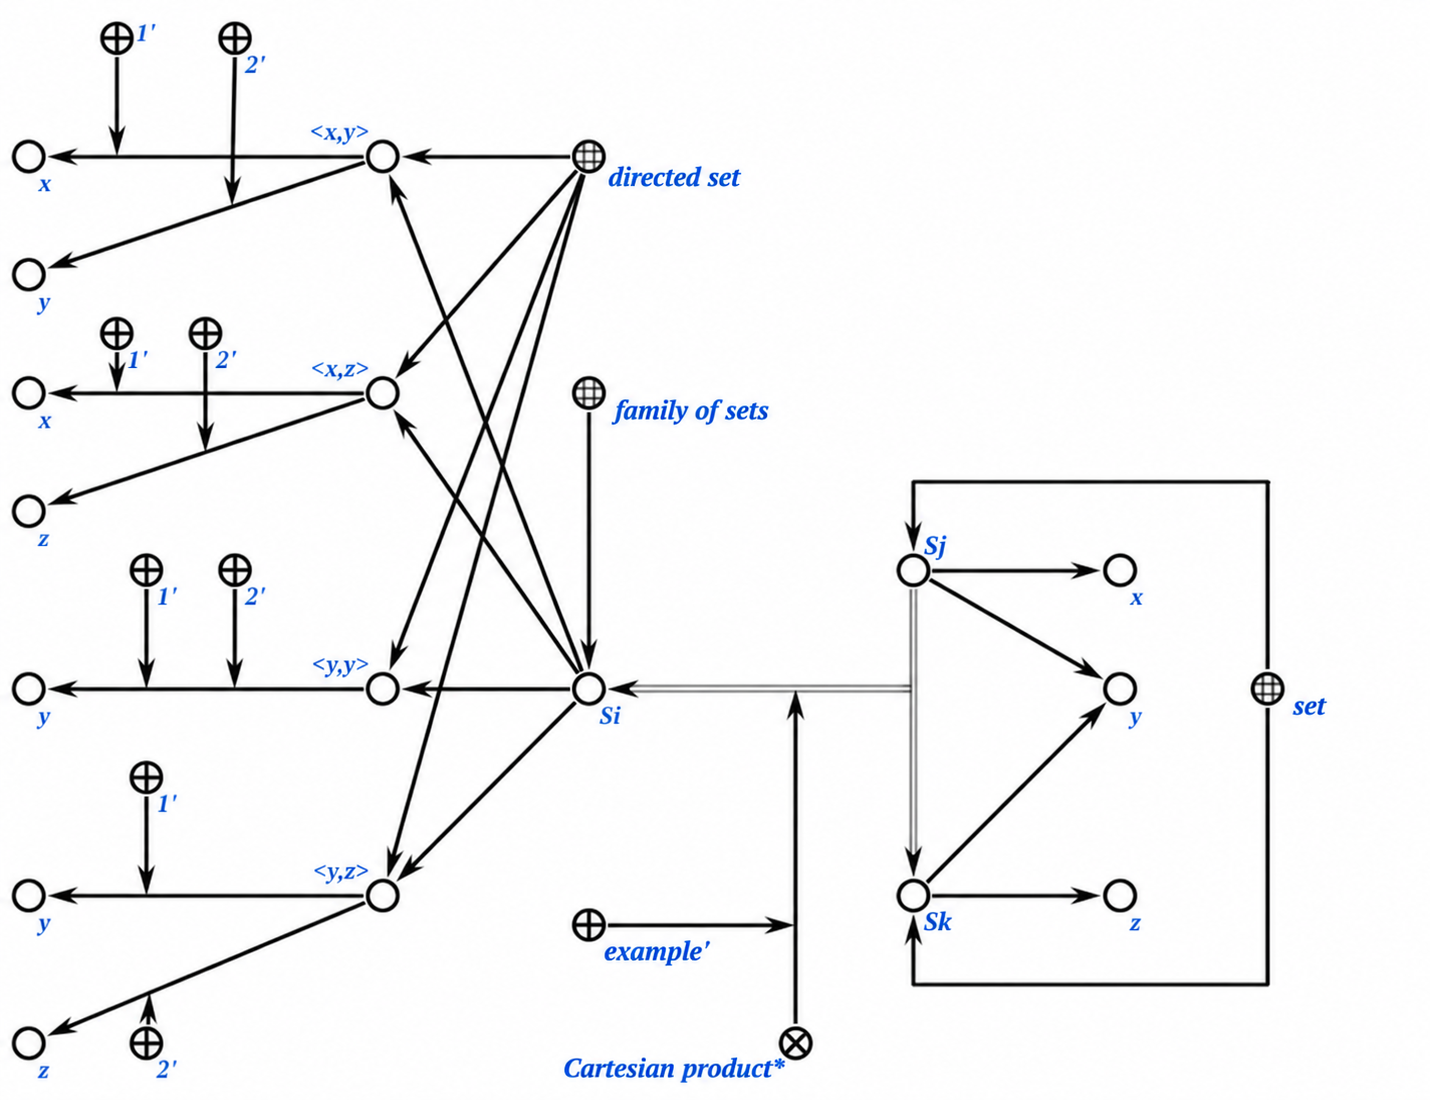
\includegraphics[width=80mm]{figures/sd_sets/cartesianMultiplication_en.png}
    \end{center}}

    \begin{scnindent}
    \scntext{explanation}{Set \textit{Si} is the Cartesian product of sets \textit{Sj} and \textit{Sk}.}
    \end{scnindent}

\end{frame}

%
\begin{frame}{\\Intersecting sets}%
\topline
\justifying
	\begin{SCn}
	\scnheader{pair of intersecting sets*}
    \scniselement{binary relation}
    \scniselement{undirected relation}

	\scntext{explanation}{\textbf{\textit{pair of intersecting sets*}} -- \textit{binary undirected relation} between two \textit{sets} with a nonempty \textit{intersection*}.}

	\scntext{definition}{\textbf{\textit{pair of intersecting sets*}} -- \textit{binary undirected relation} between two \textit{sets} that have at least one common element.}
	\end{SCn}
\vspace{1em}
\end{frame}

\begin{frame}%

   \scnrelfrom{example description}{
   \begin{center}
   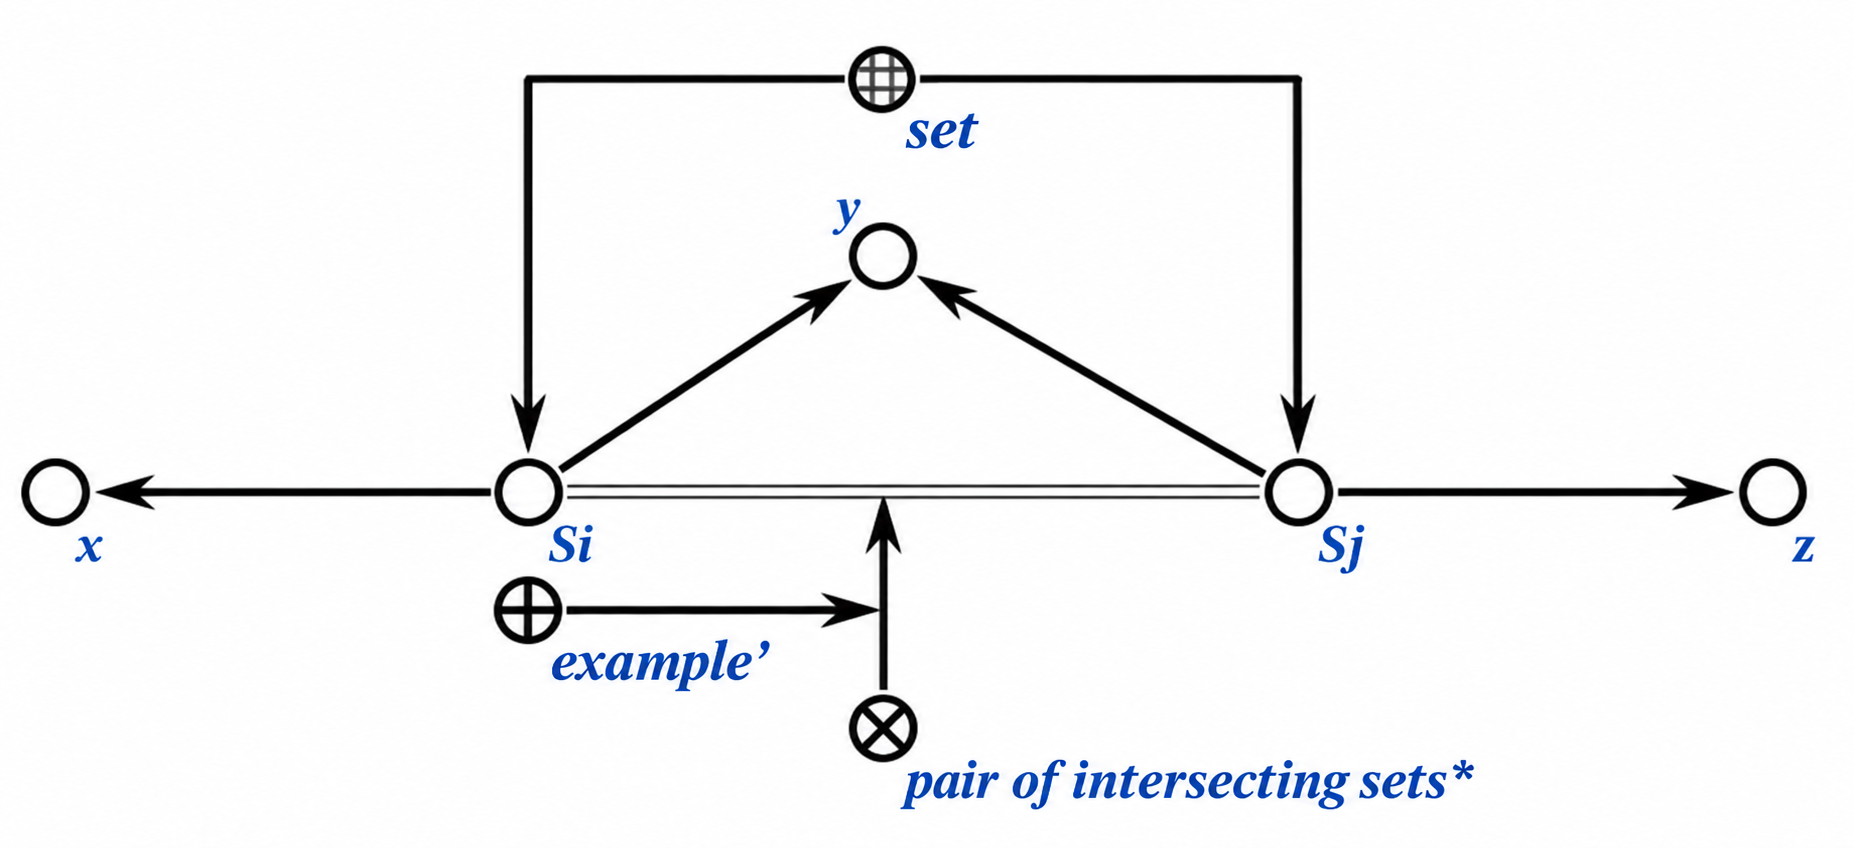
\includegraphics[width=80mm]{figures/sd_sets/pairOfIntersectingSets_en.png}
   \end{center}}

   \begin{scnindent}
   \scntext{explanation}{Set \textit{Si} and set \textit{Sj} form a pair of intersecting sets.}
   \end{scnindent}

   \scnrelfrom{illustration}{
   \begin{center}	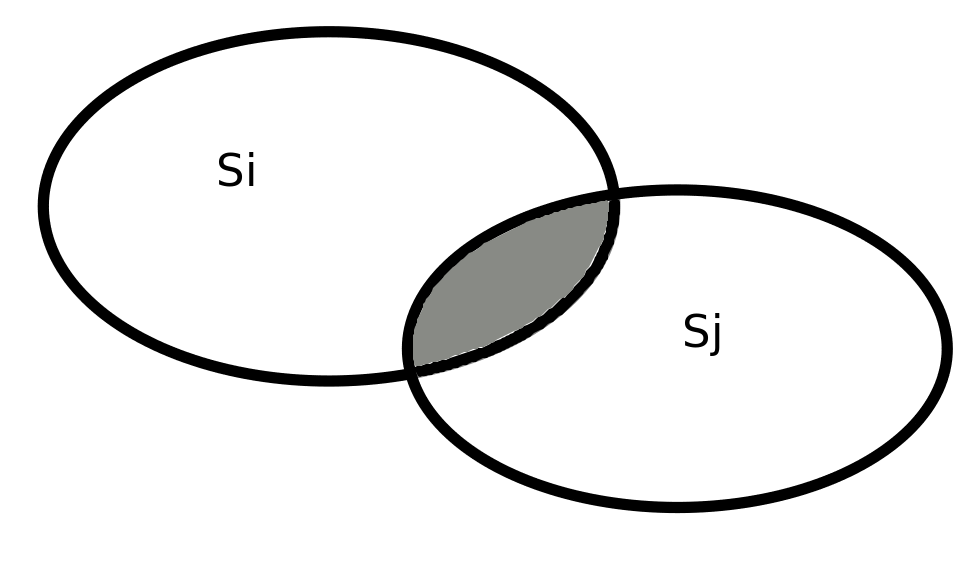
\includegraphics[width=40mm]{figures/sd_sets/pairOfIntersectingSets2.png}
   \end{center}}
\vspace{-2em}
\end{frame}

\begin{frame}%
\topline
\justifying
\vspace{10mm}

	\begin{SCn}
	\scnheader{pairwise intersecting sets*}
	\scnidtf{family of pairwise intersecting sets*}
	\scnsuperset{intersecting sets*}
	\scniselement{relation}

    \scntext{definition}{\textbf{\textit{pairwise intersecting sets*}} is a family of sets in which every pair consists of intersecting sets, i.e., every pair has at least one common element}

    \scntext{note}{Not every \textit{family of pairwise intersecting sets*} is a \textit{family of sets with a common element*} although the converse holds.}
	\end{SCn}


\end{frame}

\begin{frame}%

      \scnrelfrom{illustration}{
	\begin{center}
		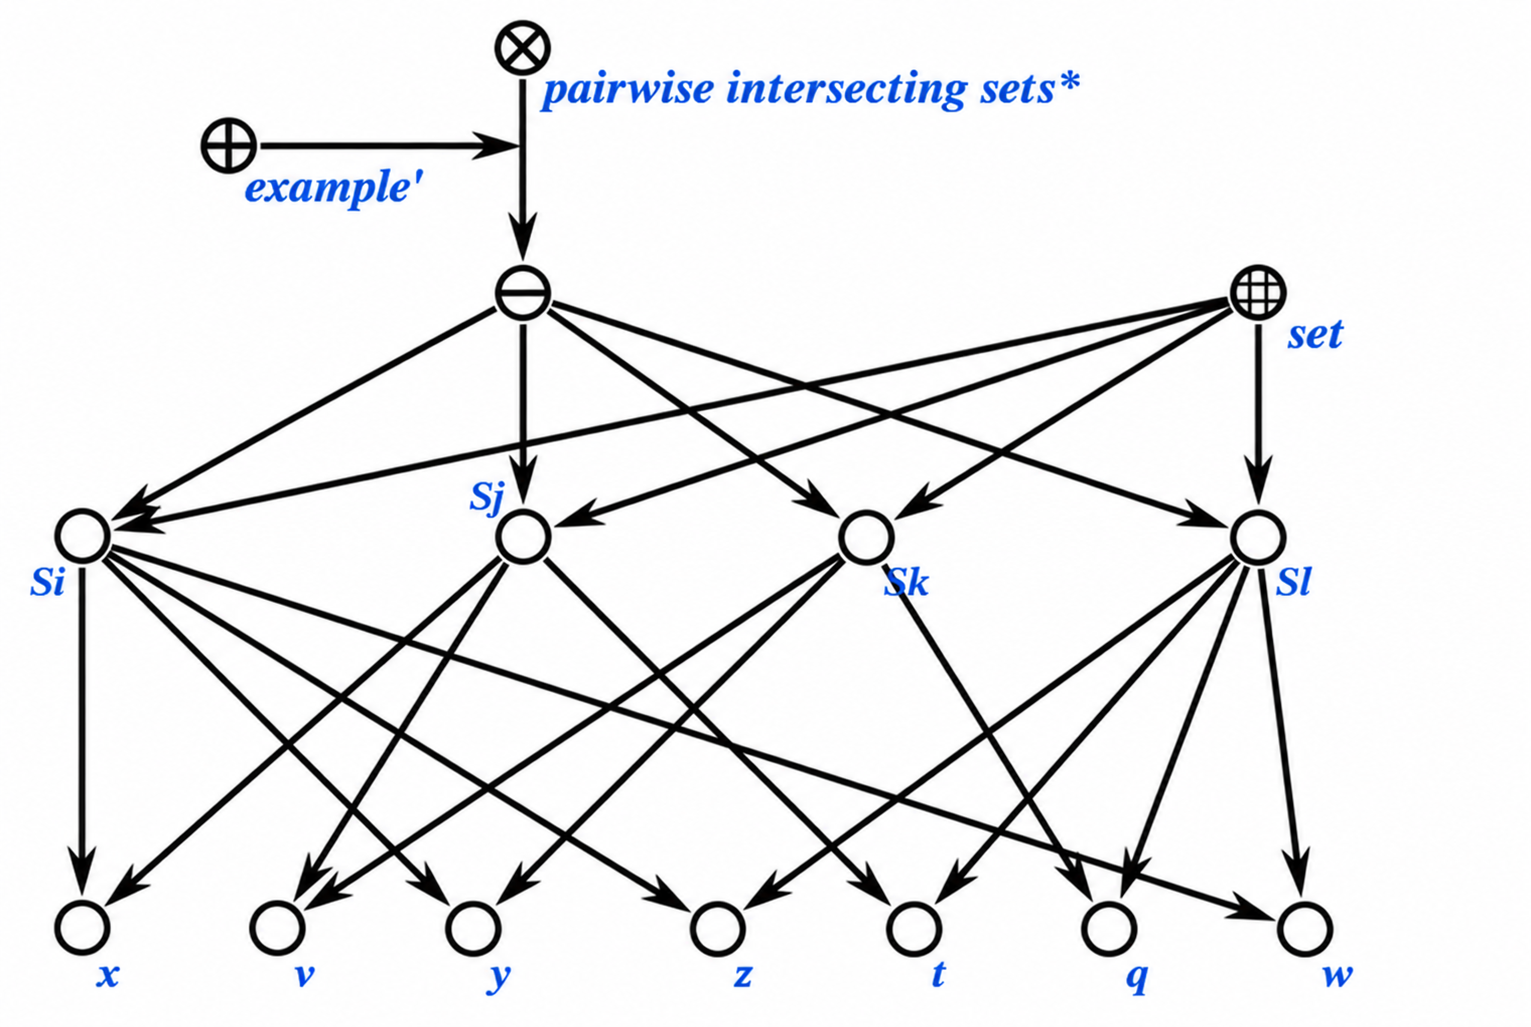
\includegraphics[width=50mm]{figures/sd_sets/pairwiseIntersectingSets_en.png}
  \end{center}}

   \begin{scnindent}
   \scntext{explanation}{Sets \textit{Si}, \textit{Sj}, \textit{Sk} and \textit{Sl} are pairwise intersecting sets.}
   \end{scnindent}


   \scnrelfrom{illustration}{
   \begin{center}
   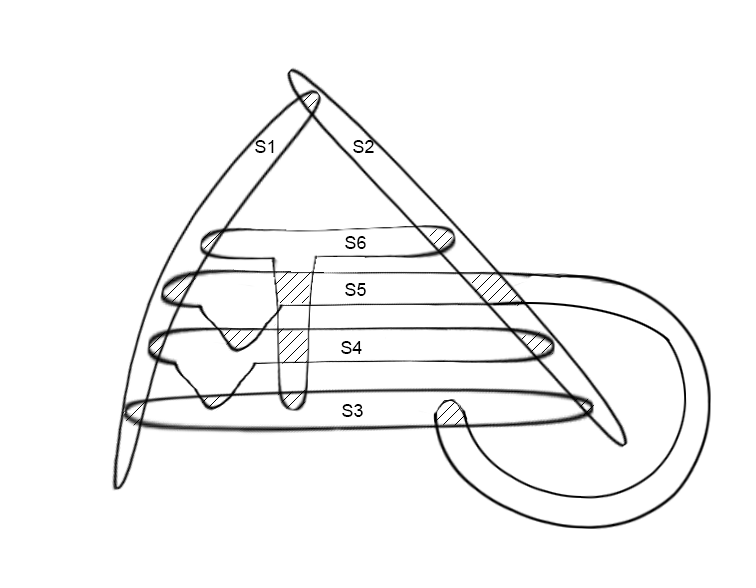
\includegraphics[width=40mm]{figures/sd_sets/pairwiseIntersectingSets2.png}
   \end{center}}

\end{frame}

\begin{frame}%
\topline
\justifying
\vspace{10mm}

	\begin{SCn}
    \scnheader{intersecting sets*}
    \scnidtf{family of sets with a common element*}
    \scnidtf{be a family of sets with a common element*}
    \scnidtf{family of sets with at least one element common to all of them*}
    \scnsuperset{pairwise intersecting sets*}

    \scntext{definition}{\textbf{\textit{intersecting sets*}} is a family of sets with at least one element common to all of them}
    \end{SCn}


\end{frame}

\begin{frame}%

   \scnrelfrom{example description}{
	\begin{center}
		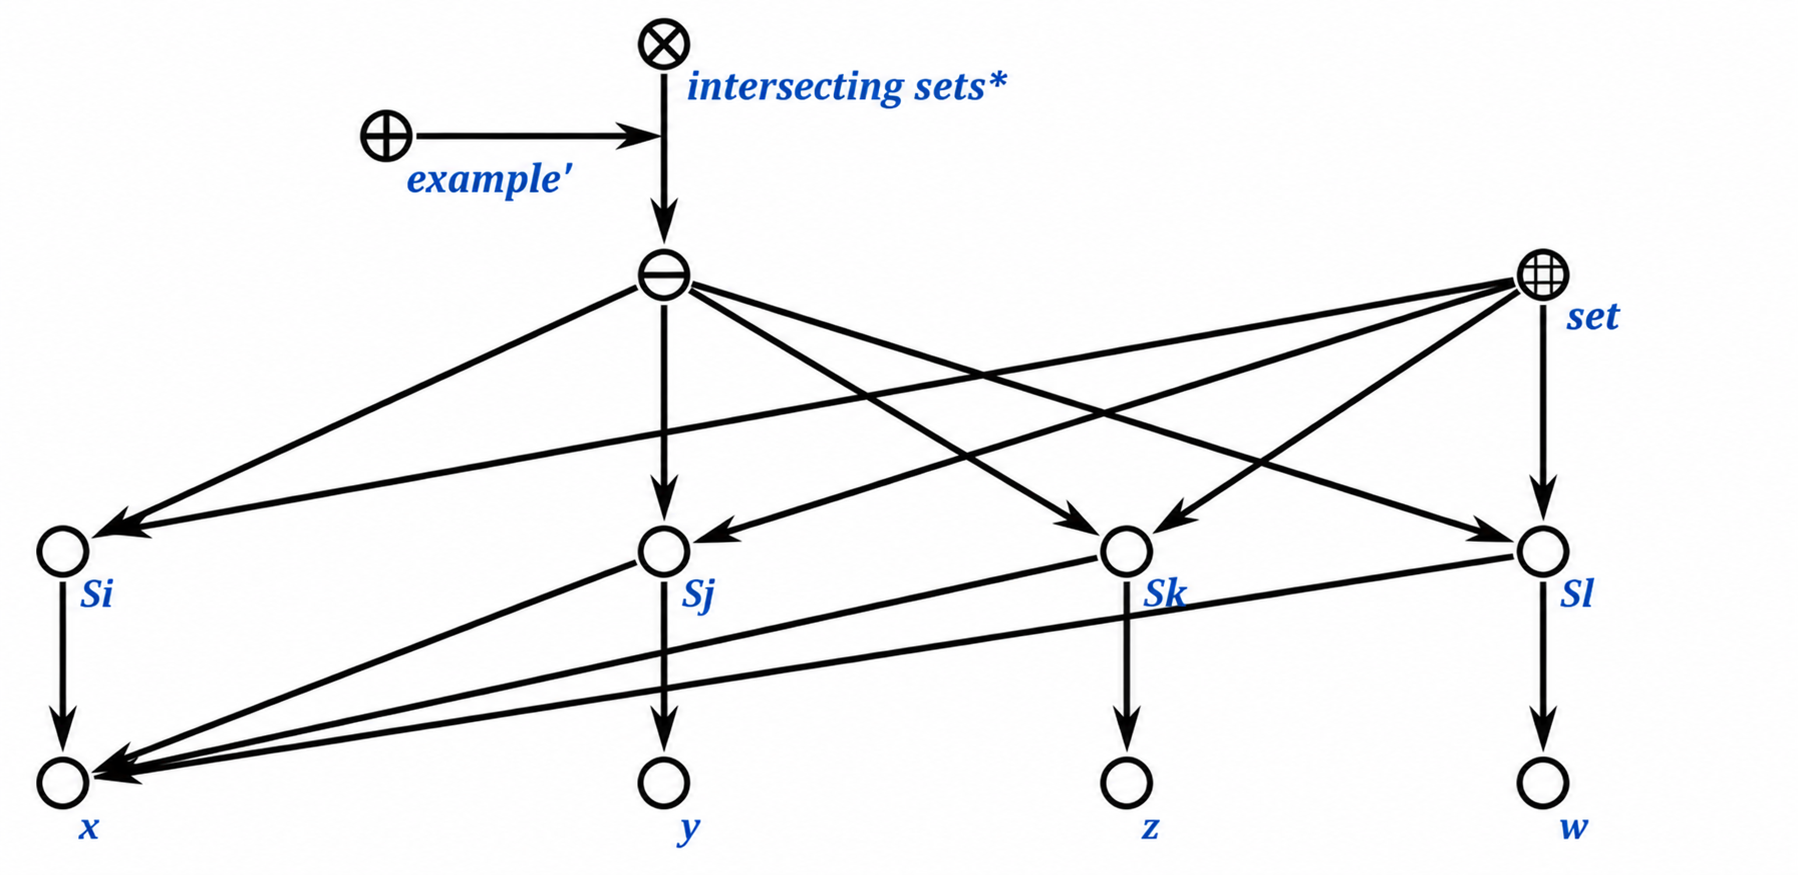
\includegraphics[width=100mm]{figures/sd_sets/intersectingSets_en.png}
  \end{center}}
  \begin{scnindent}
	\scntext{explanation}{Sets \textit{Si}, \textit{Sj}, \textit{Sk} and \textit{Sl} have a common element.}
  \end{scnindent}
\vspace{2em}
\end{frame}

\begin{frame}%
\topline
\justifying
\vspace{10mm}

	\begin{SCn}
    \scnheader{pair of disjoint sets*}
    \scniselement{binary relation}
    \scniselement{undirected relation}

    \scntext{definition}{\textbf{\textit{pair of disjoint sets*}} is a \textit{binary undirected relation} between two \textit{sets} whose \textit{intersection*} is the empty set.}
	\end{SCn}


\end{frame}

\begin{frame}%

       \scnrelfrom{example description}{
	\begin{center}
		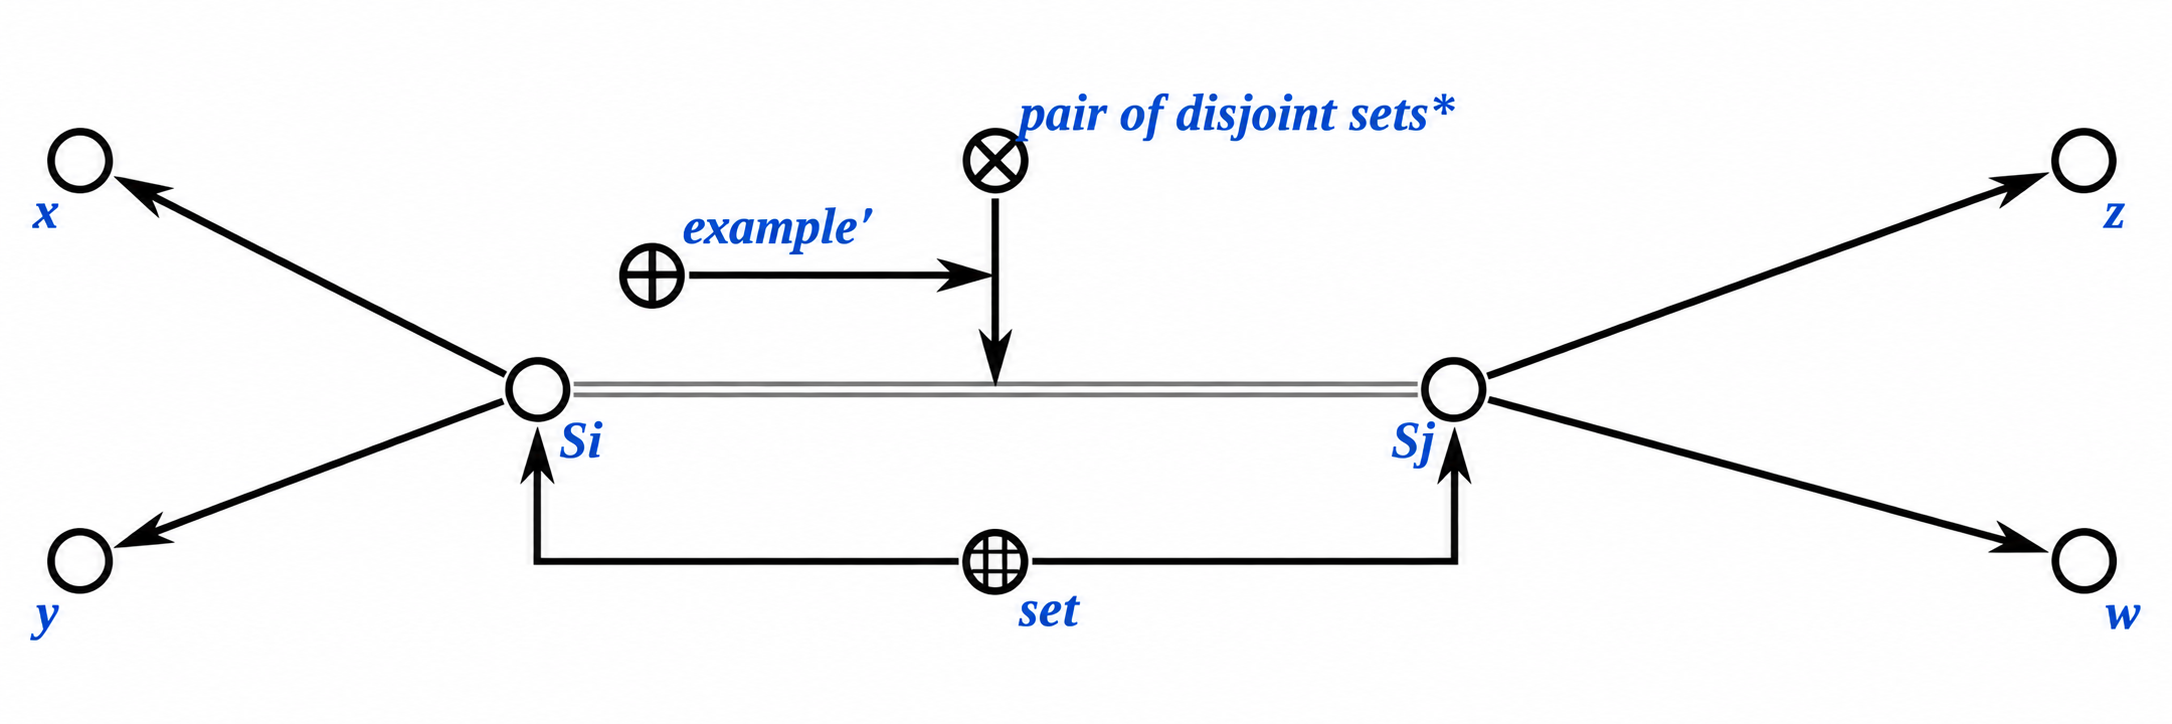
\includegraphics[width=90mm]{figures/sd_sets/pairOfNonIntersectingSets_en.png}
   \end{center}}


   \begin{scnindent}
	\scntext{explanation}{Sets \textit{Si} and \textit{Sj} form a pair of disjoint sets.}
   \end{scnindent}

   \scnrelfrom{illustration}{
	\begin{center}
		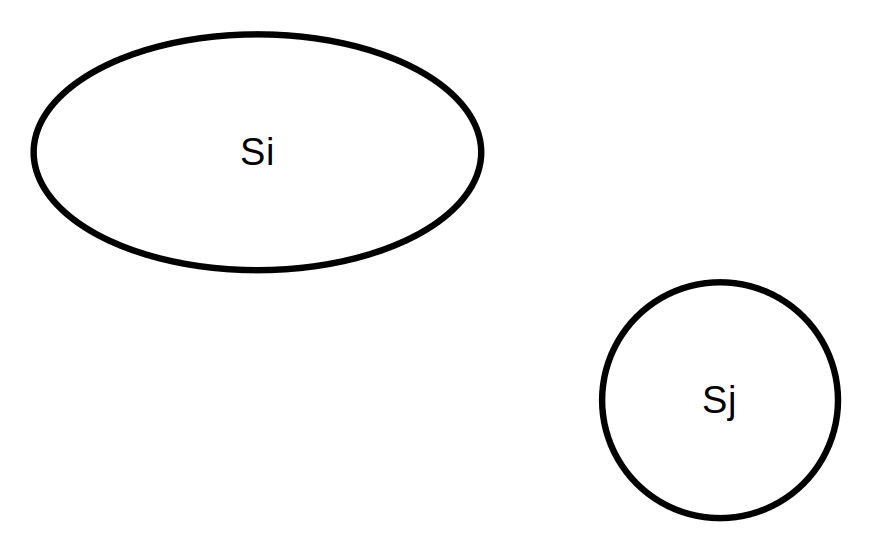
\includegraphics[width=40mm]{figures/sd_sets/pairOfNonIntersectingSets2.png}
   \end{center}}



\end{frame}

\begin{frame}%
\topline
\justifying
\vspace{10mm}

	\begin{SCn}
	\scnheader{pairwise disjoint sets*}
    \scnidtf{family of pairwise disjoint sets*}
    \scnsubset{sets with an empty total intersection*}
    \scntext{definition}{\textbf{\textit{pairwise disjoint sets*}} is a family of sets in which every pair is disjoint, i.e., no pair has a common element}
	\end{SCn}


\end{frame}

\begin{frame}%
    \scnrelfrom{illustration}{
    \begin{center}	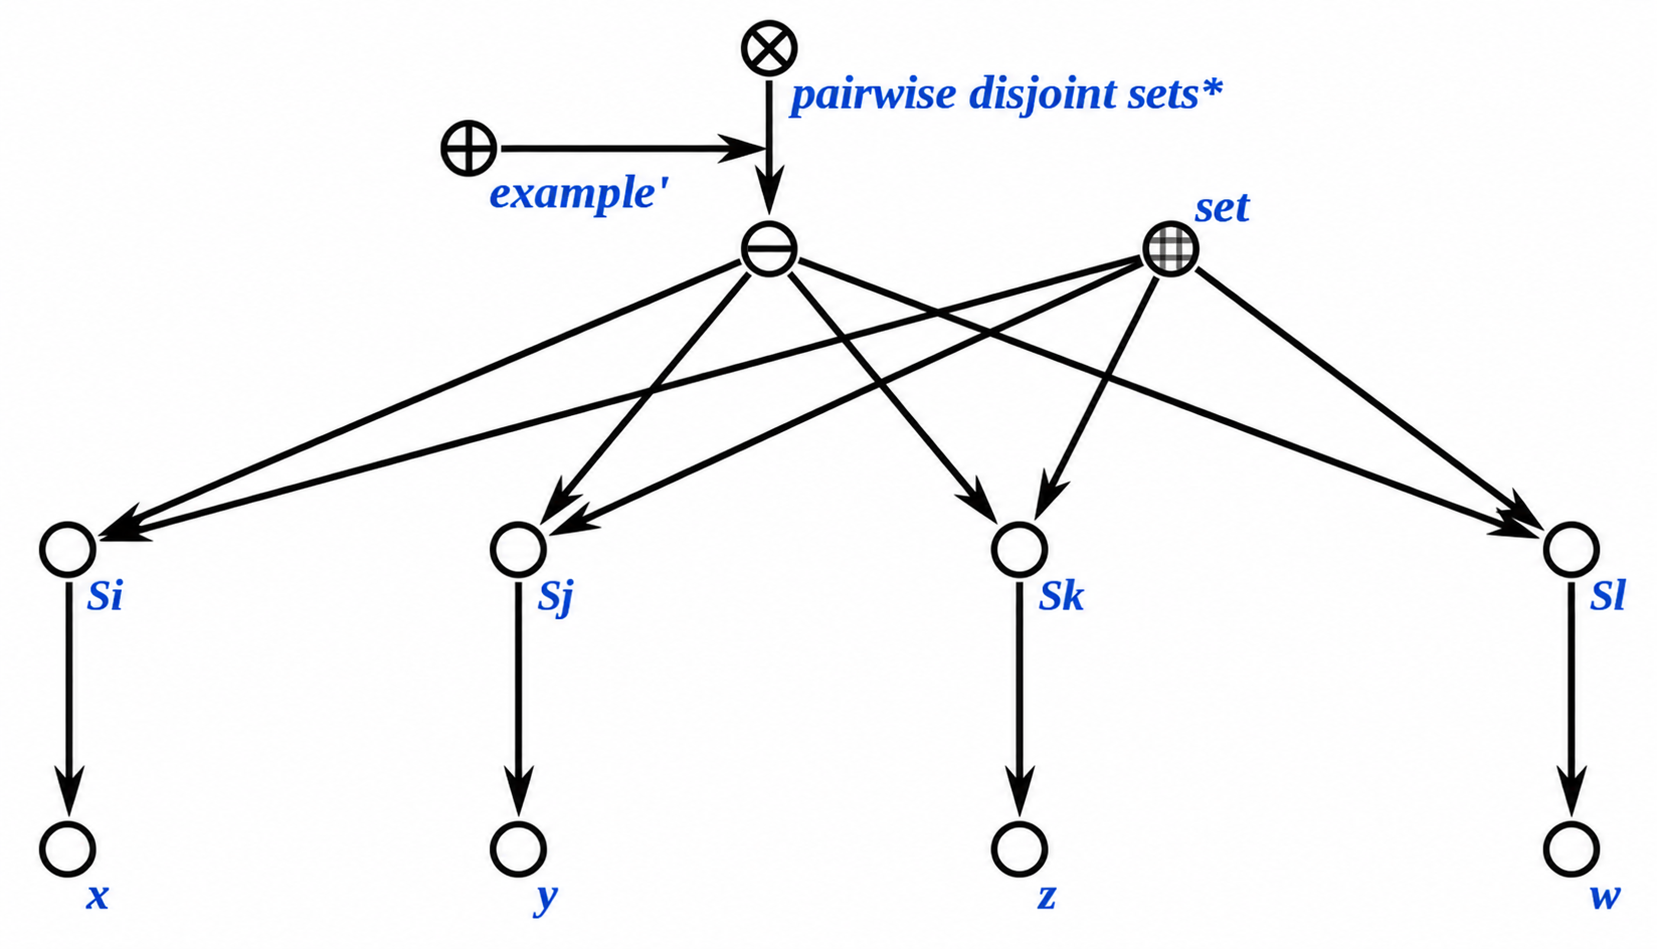
\includegraphics[width=90mm]{figures/sd_sets/pairwiseNonIntersectingSets_en.png}
    \end{center}}

    \begin{scnindent}
    \scntext{explanation}{Sets \textit{Si}, \textit{Sj}, \textit{Sk} and \textit{Sl} are pairwise disjoint sets.}
    \end{scnindent}

\end{frame}

\begin{frame}%
\topline
\justifying
\vspace{10mm}

	\begin{SCn}
    \scnheader{sets with an empty total intersection*}
    \scnidtf{family of sets with an empty total intersection*}
    \scnidtf{be a family of sets with an empty total intersection*}
    \scntext{definition}{\textbf{\textit{sets with an empty total intersection*}} is a family of sets with no element common to all of them}
	\end{SCn}


\end{frame}

\begin{frame}
    \scnrelfrom{illustration}{
    \begin{center}
	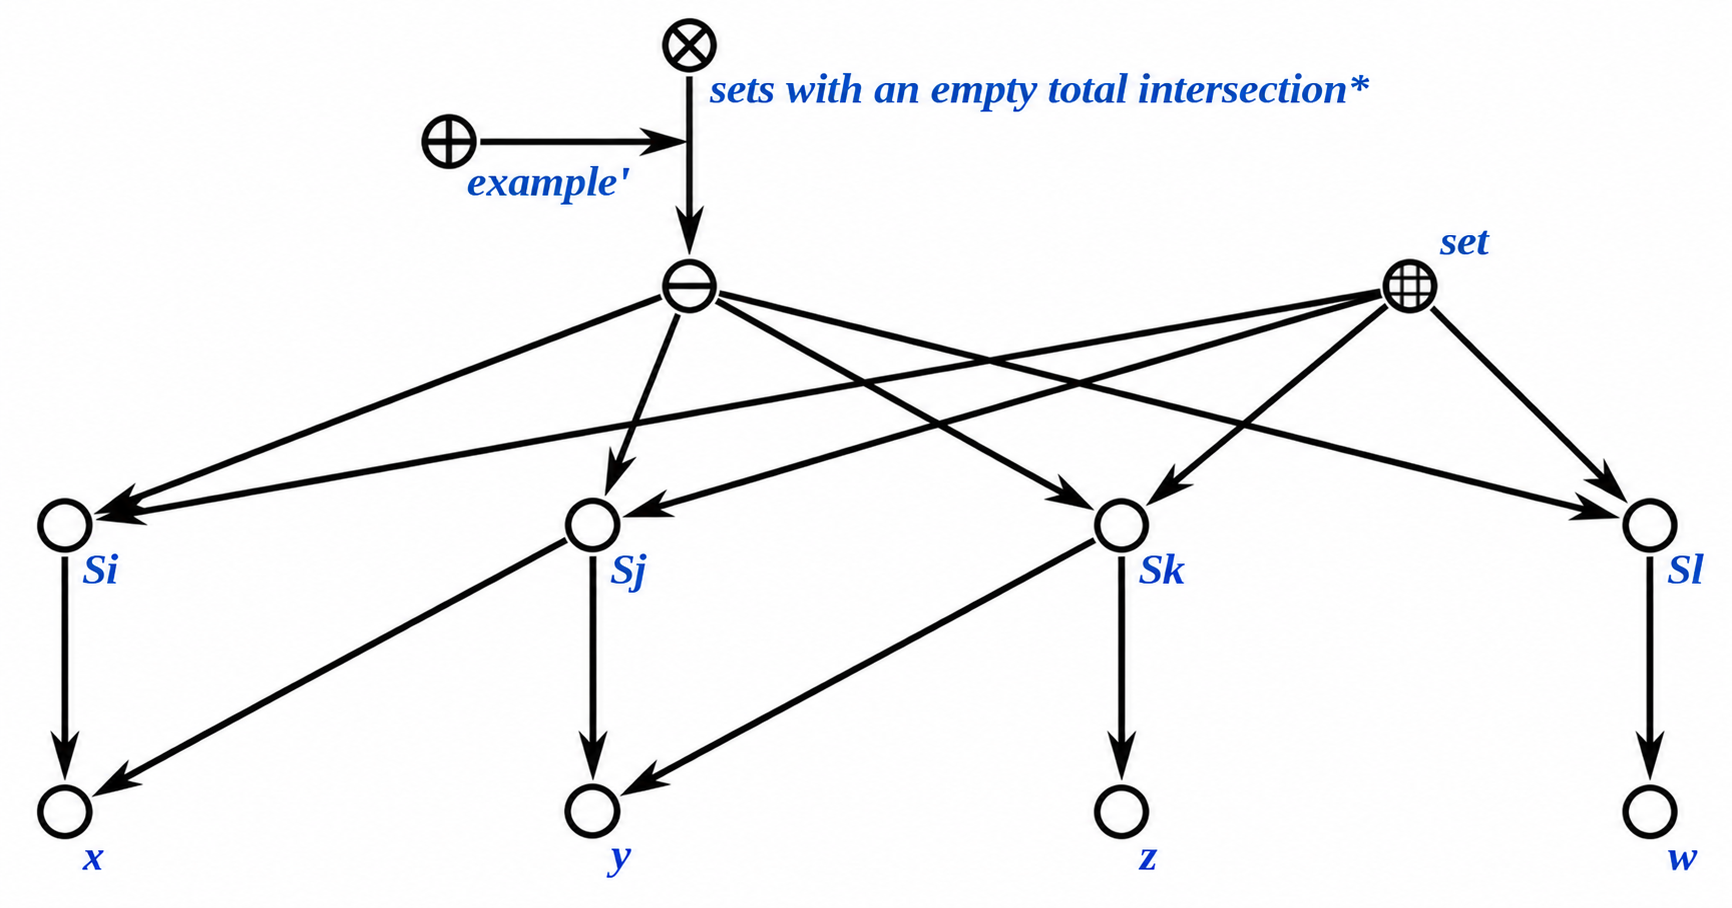
\includegraphics[width=90mm]{figures/sd_sets/nonIntersectingSets_en.png}
    \end{center}}

	\scntext{explanation}{Sets \textit{Si}, \textit{Sj}, \textit{Sk} and \textit{Sl} have an empty total intersection.}

\end{frame}
